\documentclass[11pt,a4paper]{article}

% ------------------------------------------------------------------ packages
\usepackage[a4paper,top=2.4cm,bottom=2.4cm,left=2.5cm,right=2.5cm]{geometry}
\usepackage[T1]{fontenc}
\usepackage[utf8]{inputenc}
\usepackage{mathpazo}
\usepackage{microtype}
\renewcommand{\ttdefault}{pcr}
\usepackage{amsmath,amssymb,bm}
\usepackage{graphicx}
\usepackage{booktabs,tabularx,array}
\usepackage[font=small,labelfont=bf,margin=0.5cm]{caption}
\usepackage{subcaption}
\usepackage{enumitem}
\usepackage{xcolor}
\usepackage[numbers,sort&compress,round]{natbib}
\usepackage{placeins}
\usepackage[hidelinks]{hyperref}
\usepackage[capitalise,noabbrev]{cleveref}
\usepackage{titlesec}
\usepackage{fancyhdr}

\graphicspath{{figures/}}
\setlist{itemsep=2pt,topsep=4pt}
\titleformat{\section}{\large\bfseries}{\thesection}{0.8em}{}
\titleformat{\subsection}{\normalsize\bfseries}{\thesubsection}{0.8em}{}
\titleformat{\paragraph}[runin]{\normalsize\bfseries}{}{0em}{}[.]
\titlespacing*{\paragraph}{0pt}{6pt}{0.6em}
\setcounter{secnumdepth}{3}

\pagestyle{fancy}
\fancyhf{}
\renewcommand{\headrulewidth}{0pt}
\fancyfoot[C]{\small\thepage}
\fancyhead[R]{\small\itshape Steering an attractor}

\crefname{appendix}{Appendix}{Appendices}

% ------------------------------------------------------------------ notation
\newcommand{\vect}[1]{\bm{#1}}
\newcommand{\tr}{\operatorname{tr}}
\newcommand{\pull}{\mathrm{pull}}
\newcommand{\kl}{\texttt{kl\_co\_scale}}

\title{\textbf{Steering an attractor:\\[2pt] what latent dynamics models can and cannot tell us\\ about controlling a neural circuit}}
\author{Samridh Tiwari\\[2pt]
\small Department of Physics, Indian Institute of Technology Bombay\\
\small B.Tech Project (PH587), supervised by Prof.\ Amitabha Nandi}
\date{November 2026}

\begin{document}
\maketitle
\thispagestyle{empty}

% ==================================================================== ABSTRACT
\begin{abstract}
\noindent
Latent dynamics models such as LFADS are fitted to population recordings to find the computation a circuit performs, and increasingly to decide how the circuit could be controlled. In earlier work on mouse primary motor cortex (M1), an LFADS model showed what looked like a continuous attractor holding the plan for a lever pull, yet an optimal (LQR) controller acting through the model's four inferred input channels removed only 0.1\% of the error. We test the explanation given at the time, that four channels are too few to control a 128-dimensional state, using networks where the truth is known and public monkey data. A recurrent ``teacher'' network trained to load, hold and release a plan plays the role of the circuit. Models are fitted only to Poisson spikes generated from it: a simplified LFADS-style ``student'', and full LFADS built from lfads-torch.
We report five results. (i) The number of channels is not the limit: on the teacher a single, well aimed channel has 100\% of the behavioural authority of pushing on all 100 units, and the best direction is the left eigenvector of the slow mode, $24^\circ$ from the line of states. (ii) Inferred channels are poorly aimed. The simplified student's channels reach 15--51\% of full authority. Full LFADS fits the spikes far better (single-trial rate $R^2$ 0.94--0.96) but its channels reach only 0.04--0.8\%, below random (6\%), so that an LQR controller acting through them removes 0.4--6\% of the error even at a fair effort cost; on the MC\_Maze dataset the figure is 0.3--0.5\%, against 100\% for the best four channels. The cause is the gated generator: the units that hold the memory have closed update gates, and the same gates shut out the input, so 74--98\% of the behavioural sensitivity sits on units that receive at most 3\% of the controller's push. (iii) The fitted models do not keep the plan as the circuit does. A swap test shows that the simplified student is handed the plan by its controller at the go cue, while full LFADS writes the plan into its initial state, where it can be read before the plan cue has happened ($R^2$ 0.96--0.99 on held-out trials), and therefore also reports an attractor for a teacher whose plan is held by a sustained input. Fixed-point analysis finds up to 21 marginal directions out of 64 where the circuit has one. (iv) The mechanism a model reports follows its built-in assumption, and held-out prediction does not reveal which assumption is right. (v) Two practical traps: with a causal initial condition LFADS learned to recognise its training trials from noise and recall their plans, which fails on new trials, and with its controller running LFADS undoes any perturbation of its state.
For the original result this means that the 0.1\% most likely reflects the fitted model, in particular its gated generator, rather than the cortex. We propose inexpensive checks (swap and shift tests, plan-before-cue decoding, held-out trials, and inferred channels compared with random ones) that can be run on any fitted model.
\end{abstract}

\vspace{0.5em}
{\raggedright\noindent\textbf{Keywords:} latent dynamics models; LFADS; continuous attractors; controllability; non-identifiability; motor cortex; non-normal dynamics.\par}

\newpage
\tableofcontents
\newpage

% ==================================================================== 1 INTRODUCTION
\section{Introduction}\label{sec:intro}

Population recordings from motor cortex are well described by low-dimensional dynamics \citep{churchland2012,vyas2020}, and latent dynamics models such as LFADS \citep{sussillo2016,pandarinath2018} fit a recurrent network, the generator, to single-trial spikes. The fitted generator is then studied as a stand-in for the circuit: its fixed points and slow directions are taken as evidence for attractors \citep{sussillo2013,khona2022}, and its inputs and sensitivities are used to reason about how the circuit could be perturbed.

This project started from one such analysis. During a summer research internship at Purdue (SURF), LFADS was fitted to M1 recordings from mice performing a cued lever pull. The fitted 128-unit generator showed a continuous-attractor-like structure: at its fixed points about 33 of 128 Jacobian eigenvalues were marginal and 95 were stable. A time-varying LQR controller acting through the model's four inferred input channels was then asked to steer it, and it reduced the error by only 0.1\%. The explanation offered at the time was that four channels have negligible authority over a 128-dimensional state. That explanation was never tested, and at least three explanations fit the single number equally well (\cref{fig:boats}):
\begin{enumerate}
  \item \emph{Dimension}: too few channels. Prediction: more channels fix it.
  \item \emph{Parameterisation}: the inferred channels were fitted to explain spikes, not to move anything, so their direction is arbitrary. Prediction: the same number of well aimed channels does far better.
  \item \emph{Geometry}: the circuit's own input pathways do not point where the held plan can be moved, and the inferred channels copy that. Prediction: even the true inputs steer the held plan poorly.
\end{enumerate}
Each explanation points to a different design for a future stimulation experiment. Separating them needs curves (authority against channel number, penalty and aim), and the true answer must be known. We therefore rebuilt the pipeline on recurrent networks whose dynamics are known and then checked the main result on public monkey data. No data from the Purdue laboratory is used anywhere in this report.

While doing so we found that a more basic assumption fails: the fitted model does not necessarily keep the plan in its dynamics at all. This led to the second half of the report, which asks where a fitted model keeps the plan, whether that is decided by the data or by the model's assumptions, and how it can be tested. Most of the analysis uses a simplified LFADS that could be fitted many times; in the final part we repeat the central tests with the full LFADS model of lfads-torch, the implementation used in SURF. That model reproduces the SURF observations closely and shows why its channels could not steer.

\paragraph{Contributions}
\begin{itemize}
  \item A behavioural-authority measure, computed exactly by back-propagation, that equals the error an LQR controller removes (\cref{sec:authority}), and a comparison of inferred channels against random and best channels of the same number.
  \item Evidence on known networks and on MC\_Maze that inferred input channels are poorly and inconsistently aimed for steering, while a few well aimed channels suffice (\cref{sec:res-teacher-steer,sec:res-aim,sec:res-mc}).
  \item The observation that the best push is off the attractor in a non-normal network, and that a mean-difference ``behavioural axis'' and ridge decoders cannot find it (\cref{sec:res-axis}).
  \item Three tests of where a fitted model keeps the plan (swap, shift and persistence), showing that free LFADS-style students supply the plan through their controller whether or not the circuit has an attractor (\cref{sec:res-plan}).
  \item A $2\times2$ experiment (two circuits $\times$ two model assumptions) showing that the reported mechanism follows the assumption, and that held-out prediction prefers the wrong mechanism (\cref{sec:res-toldwhen}).
  \item A replication with full LFADS showing that its inferred channels have far less authority than random channels because its gated generator shuts the input out of its memory, that it writes the plan into its initial state before the plan cue, and that it can memorise training trials (\cref{sec:res-lfads-fit,sec:res-lfads-auth,sec:res-lfads-plan}).
\end{itemize}

% ==================================================================== 2 BACKGROUND
\section{Background and related work}\label{sec:background}

\paragraph{Continuous attractors} A circuit that holds a continuous quantity, such as eye position or the strength of an upcoming movement, needs a direction in its state space along which activity neither grows nor decays. A network with a line of such steady states is a line attractor \citep{seung1996,khona2022}. Exact line attractors need fine-tuned connections; real and trained networks usually leak slowly towards a few stable points instead \citep{brody2003}. In mouse anterior lateral motor cortex, perturbations argue for a few discrete attractors rather than a line \citep{inagaki2019}, and attractor dynamics make a held choice robust to distracting pushes \citep{finkelstein2021}. Persistent delay activity in that area also depends on a loop with the thalamus \citep{guo2017}.

\paragraph{Dynamics and inputs in motor cortex} Preparatory activity sets an initial state from which movement activity unfolds \citep{churchland2012,vyas2020}, but motor cortex is not autonomous: silencing thalamic input during a reach disrupts the cortical pattern \citep{sauerbrei2020}. Whether M1 drives or mostly reflects a practised movement depends on the task \citep{guo2015,kawai2015}.

\paragraph{Latent dynamics models and identifiability} LFADS infers a per-trial initial state and, optionally, a controller that supplies inputs to the generator whenever the generator cannot explain the data; a penalty (\kl) sets how freely these inputs can be used \citep{sussillo2016,pandarinath2018}. The split between dynamics and inputs is known to be ill-posed \citep{sussillo2016}. \citet{malonis2026} showed on toy networks with known inputs that transient inputs are recovered more reliably than sustained ones, and that agreement across an ensemble of fits diagnoses when inferred inputs can be trusted. The Computation-through-Dynamics Benchmark \citep{versteeg2025} calls the failure ``dynamical misattribution'' and shows that inferred inputs depend strongly on the input prior and its penalty. Residual dynamics \citep{galgali2023} fits dynamics to trial-to-trial deviations and shows how temporally correlated upstream input biases eigenvalue estimates. Models are usually evaluated by co-smoothing, the prediction of held-out neurons \citep{pei2021}, and attractors are found by fixed-point analysis \citep{sussillo2013}.

\paragraph{Controllability} Whether a set of inputs can move a system where we want is the classical controllability question \citep{kalman1960}; the controllability Gramian measures how much change a unit of input energy buys in each direction. It has been applied to brain networks \citep{gu2015}, and motor preparation has been described as optimal control of cortex through thalamic input \citep{kao2021}. In non-normal systems the direction along which activity moves differs from the direction in which an input should push \citep{goldman2009,murphy2009}. Optogenetic and electrical perturbations of monkey motor cortex during reaching are the experimental counterpart of the questions asked here \citep{oshea2022}.

% ==================================================================== 3 METHODS
\section{Methods}\label{sec:methods}

\Cref{fig:pipeline} summarises the approach. All time steps are 20\,ms.

\begin{figure}[t]
  \centering
  \begin{subfigure}{\linewidth}\centering
    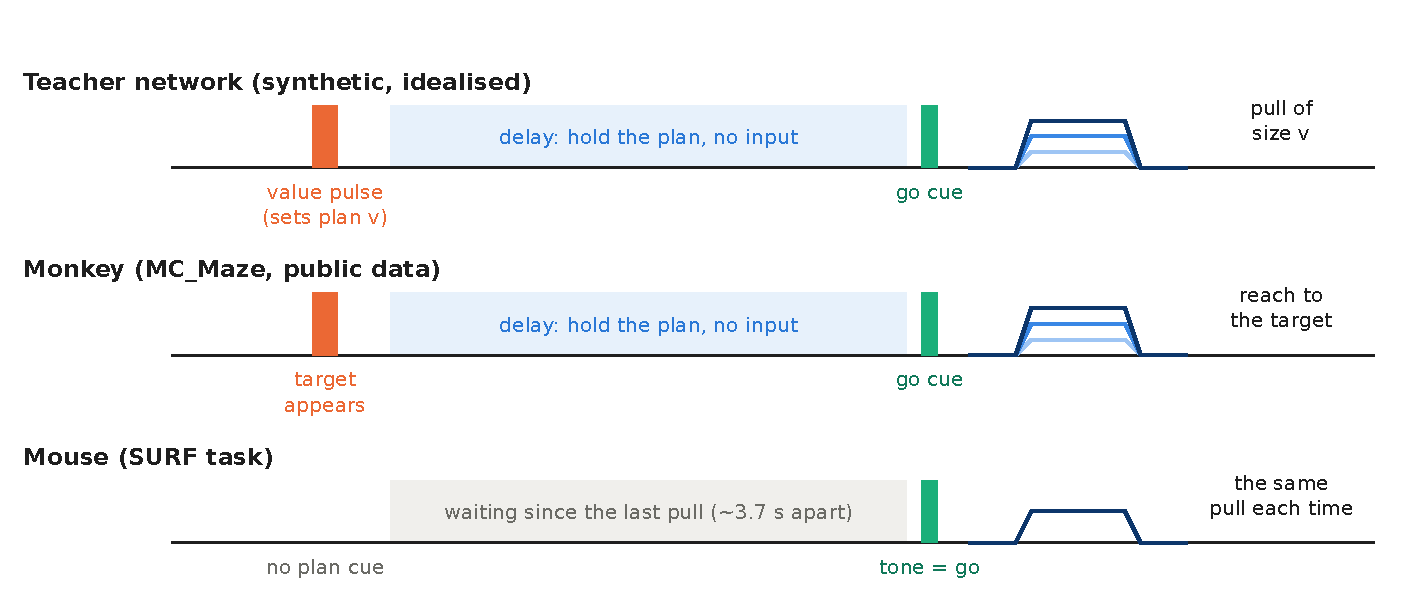
\includegraphics[width=0.92\linewidth]{d4_task.pdf}
    \caption{The task for the teacher, the monkey (MC\_Maze) and the SURF mouse.}
  \end{subfigure}\\[6pt]
  \begin{subfigure}{\linewidth}\centering
    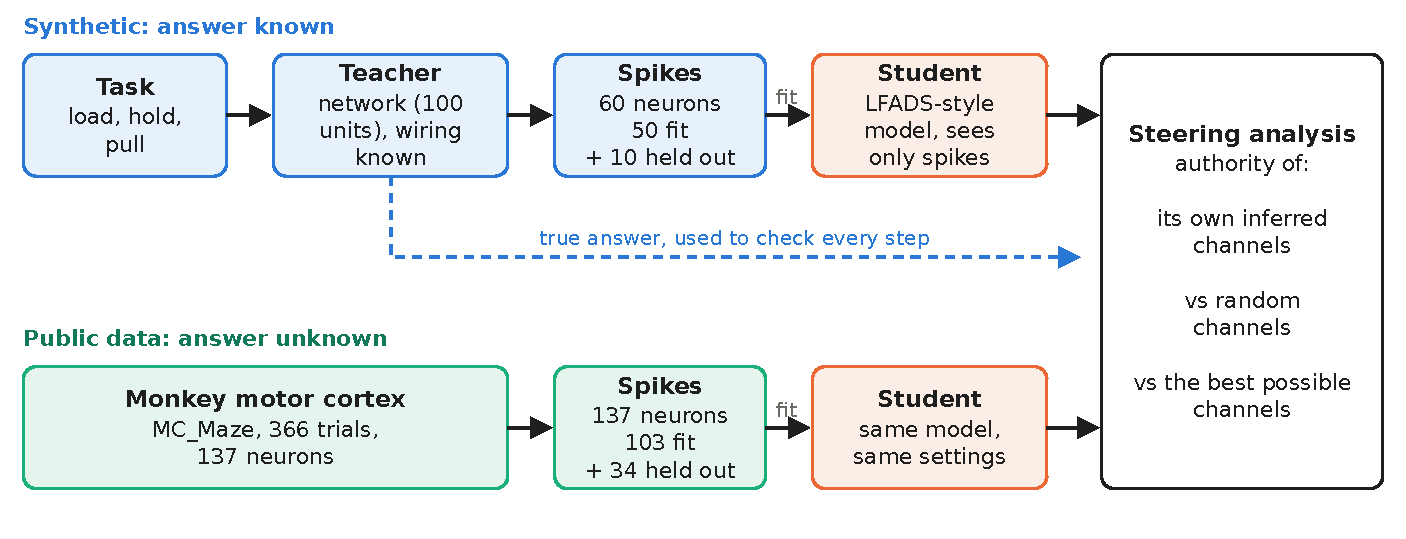
\includegraphics[width=0.92\linewidth]{d5_pipeline.pdf}
    \caption{The pipeline: the same student and analysis are used on the teacher, where the answer is known, and on public monkey data.}
  \end{subfigure}
  \caption{Overview. The teacher and the monkey load a plan, hold it through a delay and release it after a go cue. The SURF mouse task has no plan cue; the tone is the go signal and the pull is roughly the same on every trial.}
  \label{fig:pipeline}
\end{figure}

\subsection{Teacher networks}\label{sec:teacher}

The teacher is a discrete-time recurrent network of $N=100$ tanh units,
\begin{equation}
  \vect h_{t+1} = \tanh\!\left(W \vect h_t + W_{\mathrm{in}} \vect x_t + \vect b\right), \qquad y_t = \vect w_{\mathrm{out}}^\top \vect h_t + b_{\mathrm{out}},
\end{equation}
with two input lines $\vect x_t$ (plan and go) and a lever output $y_t$. On each 150-step trial a plan $v \sim \mathcal U(0.2,1)$ is presented as a 5-step pulse of height $v$ at a random step between 10 and 20 (\emph{teacher A}). After a silent delay of 35--85 steps a 3-step go cue arrives, and the lever must rise over 8 steps to height $v$, hold for 20 steps and fall over 8. Behaviour is the \emph{pull}, the mean lever output over the 20-step plateau. Training used Adam for 6000 steps with recurrent gain 0.9 at initialisation and activity noise 0.05. A second, training-only output that reports $v$ during the delay was needed to stop the network converging to a constant average pull; it is ignored afterwards. A second network was trained identically from a different seed (\emph{teacher A2}).

To ask whether a fitted model can tell a memory held by the circuit from a plan held from outside, we also trained \emph{teacher B} on the same task, except that its plan input stays on at height $v$ throughout the delay. Teacher B needs no memory. Both teachers perform the task equally well (correlation of pull with plan 0.999 and 1.000).

\subsection{Synthetic recordings}\label{sec:data}

From each teacher we generated 256 trials of spikes from 60 artificial neurons. Each neuron's log firing rate is a random mixture of the teacher's units,
\begin{equation}
  \log r_{t,n} = \log \beta_n + \sigma\, z_{t,n} - \sigma^2/2, \qquad \vect z_t = \operatorname{standardise}(C \vect h_t),
\end{equation}
with $C$ a $60\times100$ Gaussian matrix, $\sigma=0.7$ and baseline rates $\beta_n \sim \mathcal U(0.08,0.45)$ spikes per step, and spike counts are Poisson. Fifty neurons are used for fitting and ten are held out. No noise is added to the teacher's dynamics when data are generated.

\subsection{The free student}\label{sec:student}

The student is a simplified LFADS (\cref{fig:a-student}) with a 64-unit generator, 12 factors and $k$ input channels:
\begin{equation}
  \vect g_{t+1} = \tanh\!\left(W \vect g_t + B \vect u_t + \vect b\right), \qquad \log \vect r_t = D F \vect g_t + \vect d .
  \label{eq:student}
\end{equation}
$F$ ($12\times64$) forms the factors and $D$ ($50\times12$) maps them to the recorded neurons, so the readout has rank at most 12. The columns of $B$ (the channel directions) are kept at unit length, otherwise the model could grow $B$ and shrink $\vect u$ to avoid the penalty. The initial state $\vect g_0$ and the inputs $\vect u_t$ are free parameters for every trial. The objective is the Poisson negative log-likelihood plus $\lambda\,\overline{u^2} + 10^{-5}\lVert W\rVert^2$, where the penalty $\lambda$ plays the role of LFADS's \kl{} (the scales are not comparable, since LFADS penalises a KL divergence). Each fit is 2500 Adam steps. Because the controller may add input at any time step, we call this the \emph{free} student. We sweep $\lambda \in \{10^{-4},10^{-2},0.1,1,10\}$ and $k\in\{1,2,4,8,16\}$, with three to five seeds at the main settings.

Generalisation is measured by co-smoothing: with the fitted model fixed, a Poisson readout from the 12 factors (13 parameters per neuron) is fitted to each held-out neuron, and prediction is reported in bits per spike relative to a constant-rate model \citep{pei2021}.

\subsection{The told-when student}\label{sec:toldwhen}

To test how much the results depend on the controller's freedom, we built a student with the opposite assumption. It has the same generator, factors and readout and one shared initial state, but its only inputs are locked to the two cue times of each trial:
\begin{equation}
  \vect g_{t+1} = \tanh\!\Big(W \vect g_t + \vect b + \sum_{c=1}^{2} a_{ic}\, K^{\mathrm{load}}_c\big[t - t^{\mathrm{load}}_i\big] + K^{\mathrm{go}}\big[t - t^{\mathrm{go}}_i\big]\Big).
\end{equation}
$K^{\mathrm{go}}$ is one learned go-locked waveform (lags $-3$ to $+11$) shared by all trials, so it can trigger the pull but cannot carry anything trial-specific. $K^{\mathrm{load}}_{1,2}$ are two learned waveforms (lags $-1$ to $+6$) scaled on trial $i$ by two fitted numbers $a_{ic}$; these are the only trial-specific inputs, and they end 7 steps after the plan cue. Whatever distinguishes trials at the time of the pull must therefore be carried through the delay by the generator. The assumption is correct for teacher A and wrong for teacher B. Fits use 7000 steps; with 2500 the model learned when to pull but not how hard.

\subsection{Full LFADS}\label{sec:lfads}

To check that the results do not come from the simplifications of the free student, we also fitted the full LFADS model. It was assembled from the modules of lfads-torch \citep{sedler2023}, the implementation used in SURF, with our own training loop in place of the library's training framework. A bidirectional GRU \citep{cho2014} reads the spikes of the whole trial and gives a Gaussian posterior over the initial condition. A second bidirectional GRU encodes the spikes for the controller, a GRU that also sees the previous step's factors and gives a posterior over a four-dimensional controller output $\vect u_t$. The generator is a GRU driven by $\vect u_t$; factors and the Poisson readout are as in the free student. The priors are those of lfads-torch: a Gaussian over the initial condition (variance 0.1, learned mean) and an autoregressive prior over the controller output (time constant 10 steps, learned). The loss is the Poisson reconstruction error, the two KL terms, the controller's KL weighted by \kl{}, and a small $L_2$ penalty on the recurrent weights, the last three ramped in over the first 20\% of training. Coordinated dropout (rate 0.3) stops the model from copying its input to its output \citep{keshtkaran2019}. To fit on a CPU the sizes are smaller than in SURF: generator 64 units, controller 32, factors 12, encoders 32 units per direction. Each fit is 3000 Adam steps (learning rate $4\times10^{-3}$) on batches of 64 trials.

Unlike the free student, LFADS infers the initial condition and controller output with an encoder, so it can be applied to trials it was not trained on. Each fit therefore used 192 training trials, and every test below was run on the 64 held-out trials (the co-smoothing readout was fitted on training trials only). We swept \kl{} from $10^{-6}$ to $10^{-2}$; the SURF configurations used $10^{-5}$ and $10^{-4}$.

Two variants test what the model is allowed to know. In the \emph{causal IC} variant the initial-condition encoder sees only the first 8 steps, before the earliest plan cue (step 10 to 19), using lfads-torch's own option for this. The plan then has to enter through the controller. In the \emph{not sampled} control, the controller passes its posterior mean to the generator during training instead of a random sample from the posterior.

\paragraph{Changes to the tests} Pushes are added to the generator state. The inferred channels at time $t$ are the directions $\partial\vect g_t/\partial\vect u_t$, which depend on the state; for a window we use the top four left singular vectors of these Jacobians stacked over the window. Random and best channels are defined as in \cref{sec:authority}. The tests can be run in two ways. In \emph{open loop} the generator alone is driven by the recorded controller outputs (replaying them reproduces the fitted trajectory exactly). In \emph{closed loop} the whole model runs, and the controller keeps reading the encoded spikes; a closed-loop swap gives trial $i$ the encoded spikes of trial $j$. To see when a model knows the plan, we decode the plan value $v$ from the model state at each time step with a ridge regression (cross-validated $R^2$, even and odd trials).

\subsection{Behavioural authority and its relation to LQR}\label{sec:authority}

For a small push $\vect x_t$ added to the pre-activation at time $t$, the pull changes by
\begin{equation}
  \Delta \pull \approx \sum_t \vect s_t^\top \vect x_t, \qquad \vect s_t = \frac{\partial\, \pull}{\partial \vect x_t},
\end{equation}
where the sensitivity $\vect s_t$ is computed exactly by back-propagation through the whole trial. Summing over a window gives $Q = \sum_{t\in\text{window}} \vect s_t \vect s_t^\top$, and the authority of $k$ orthonormal channels $B$ is
\begin{equation}
  G(B) = \tr\!\left(B^\top Q B\right),
\end{equation}
the controllability Gramian measured on behaviour. An LQR controller asked to shift the pull by $T$ with effort cost $\rho$ achieves exactly
\begin{equation}
  \frac{\Delta \pull}{T} = \frac{G}{G+\rho}
  \label{eq:lqr}
\end{equation}
of the target (derivation in \cref{app:derivation}), which we verified numerically against direct optimisation. Every channel set is compared with three references: $k$ random orthonormal directions (on average $k/N$ of full authority; 200 draws), the best $k$ directions (the top eigenvectors of $Q$), and pushing on every unit, $G=\tr Q$ (\emph{full authority}). We report $G(B)/\tr Q$, the \emph{fraction of full authority}, and set $\rho$ so that full actuation removes 90\% of the error (the \emph{fair} setting). Two windows are used: the 5 load steps (a positive control) and the delay, from 30 to 5 steps before the go cue. Values are medians over trials. For students, the pull is read from the generator state with a ridge decoder fitted to the teacher's lever (\cref{app:details}).

\paragraph{Whole-state goal and effort cost} To compare with an LQR targeting the full model state, we also compute the error removed when the target is an arbitrary displacement of the state 5 steps before the go cue, averaged over random targets, using the exact Jacobian of that state with respect to pushes in the delay window. We then sweep $\rho$ over seven orders of magnitude around the fair value for both goals.

\subsection{Tests of where a model keeps the plan}\label{sec:tests}

A model with a controller can keep the plan in three places: in the generator's dynamics, in controller input fed through the delay, or in controller input at the go cue. Only the first is a memory held by the circuit. Each test below is applied identically to the teacher (where the answer is known) and to the students.

\paragraph{Swap test} Trial $i$ runs normally until 8 steps after its plan pulse; from then on it receives the inputs of a randomly chosen trial $j$, aligned on the go cue (for the teacher its true inputs, for a student its inferred inputs). Over all trials we fit $\pull \approx \alpha v_i + \beta v_j + c$ and report $\alpha$, the share of the pull set by the trial's own state (\cref{fig:swap}). For MC\_Maze the reach end point replaces $v$.

\paragraph{Shift test} Twenty-five steps before the go cue the state is displaced by $0.1\,\vect m$, where $\vect m$ is the slope of a regression of state on $v$ across trials, with all inputs unchanged. The \emph{gain} is the resulting change in pull divided by the change expected from a plan increase of 0.1.

\paragraph{Persistence} The propagator $\Phi = J_{t+20}\cdots J_{t+1}$ is the product of the Jacobians along the trial's own trajectory from 30 to 10 steps before the go cue. Its eigenvalues give what is left of a small displacement after 20 steps. A memory direction has a real, positive eigenvalue near 1; rotating or sign-flipping directions are not counted. Unlike single-step eigenvalues, this does not assume the state is at a fixed point.

\paragraph{Fixed-point analysis} As in SURF, fixed points of the autonomous generator (controller off) are found from 32 delay states by minimising $\lVert f(\vect g)-\vect g\rVert^2$ \citep{sussillo2013}, kept if the residual is below $10^{-5}$, and Jacobian eigenvalues with $0.95<|\lambda|<1.05$ are counted as marginal.

\subsection{Transfer of the model's best push to the circuit}\label{sec:transfer}

To ask whether a fitted model tells us where to push the real circuit, we translate the student's sensitivity to the teacher through the recorded neurons. A teacher push $\vect y$ changes the recorded log-rates at once by $M_T \vect y$; the smallest student push with the same immediate effect is $M_S^{+} M_T \vect y$, so the model's estimate of the teacher's sensitivity is $\hat{\vect s}_T = M_T^\top (M_S^{+})^\top \vect s_S$. We compare $\hat{\vect s}_T$ with the true $\vect s_T$ over 64 trials in the delay window. A perfect model is limited only by the 50 recorded neurons not seeing all 100 units, which caps it at 87\% of full authority.

\subsection{Public data}\label{sec:mcmaze}

We used the large MC\_Maze session of the Neural Latents Benchmark \citep{pei2021}: monkey J, Utah arrays in motor and premotor cortex, delayed reaches to targets, sometimes around obstacles. Spikes were binned at 20\,ms and aligned on the go cue from $-300$ to $+800$\,ms. Successful trials with delays of at least 350\,ms were kept (366 trials), with 137 neurons firing above 1\,Hz, of which 103 were fitted and 34 held out (the benchmark's split). Students had 64 units, $k=4$ at $\lambda \in \{10^{-4},0.1\}$ (three seeds each) and $k\in\{1,16\}$ at $\lambda=0.1$ (two seeds each). Predicted log-rates were capped and the learning rate halved to avoid divergence. Behaviour is the reach end point: the $x$ and $y$ displacement of the hand over the first 400\,ms after movement onset, decoded from the generator state (cross-validated $R^2$ 0.88--0.96 for $x$, 0.75--0.79 for $y$). Sensitivity is computed for pushes in the last 300\,ms of the delay.

% ==================================================================== 4 RESULTS
\section{Results}\label{sec:results}

\subsection{The teacher holds the plan on an approximate line attractor}\label{sec:res-teacher}

Teacher A performs the task with lever $R^2=0.999$ and pull--plan correlation 0.999 (\cref{fig:teacher}a). Delay states lie on a thin curved thread (\cref{fig:a-thread}): the first three principal components carry 86\%, 11\% and 2\% of the variance and the participation ratio is 1.25 (\cref{fig:teacher}b). Linearised in the middle of the delay, the dynamics have one eigenvalue at 1.00 along the thread and the next at 0.64, so displacements off the thread decay within a few steps (\cref{fig:teacher}c). The attractor leaks: left in silence for 60\,s (3000 steps), states collect at about five points, but the drift during a real delay is negligible (median speed $6\times10^{-7}$ per step).

\begin{figure}[t]
  \centering
  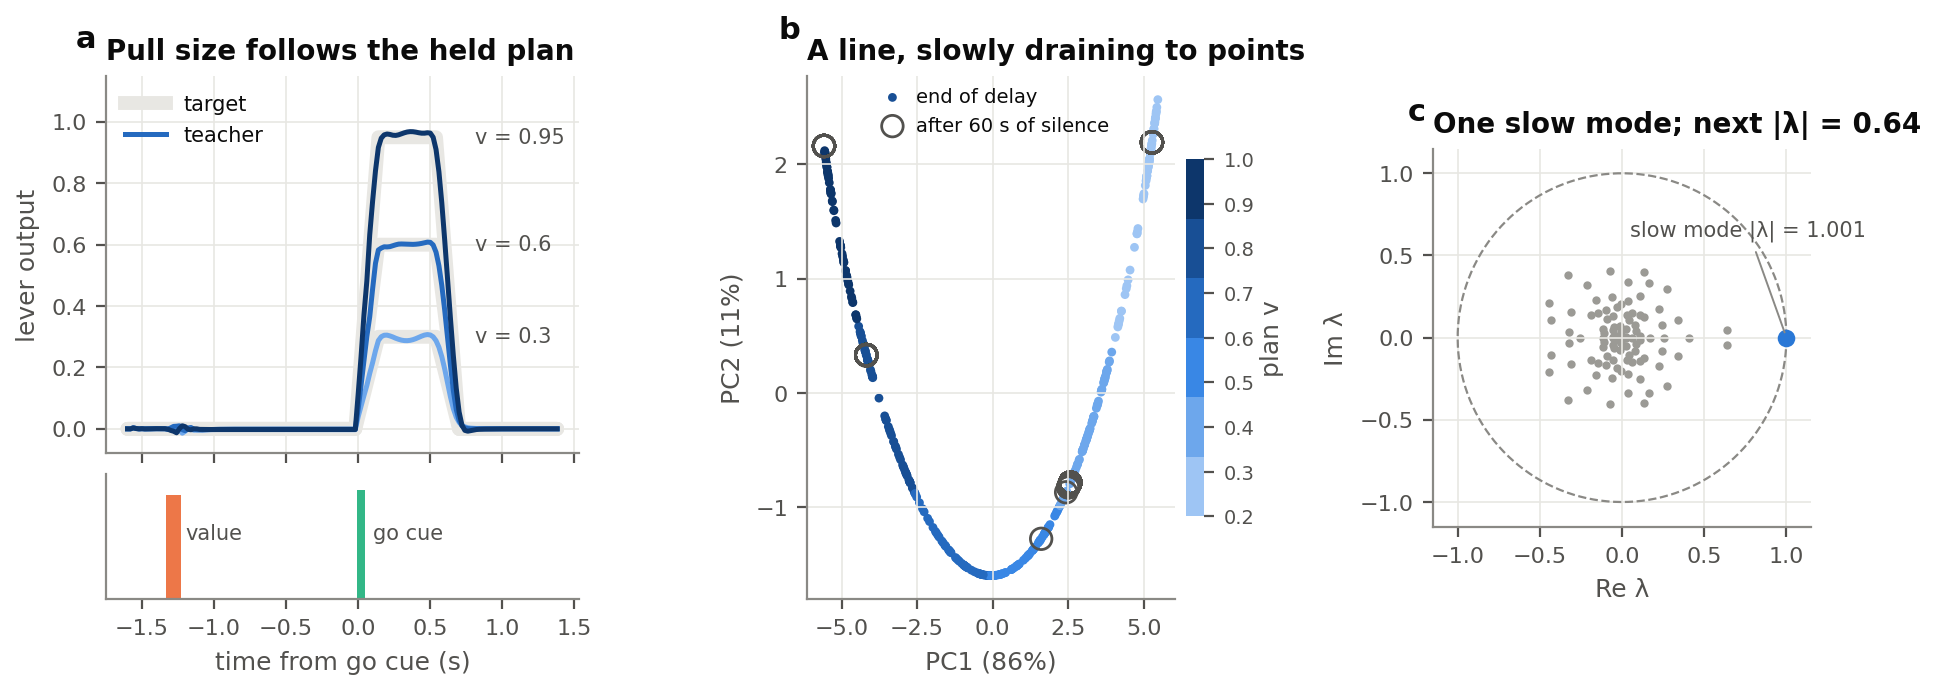
\includegraphics[width=\linewidth]{fig1.png}
  \caption{The teacher. (a) Lever output for three plans, with the plan pulse and go cue below. (b) States at the end of the delay, coloured by plan $v$, on the first two principal components; open circles show where states end up after 60\,s of silence. (c) Eigenvalues of the linearised dynamics in the middle of the delay: one slow mode on the unit circle, the rest well inside.}
  \label{fig:teacher}
\end{figure}

\subsection{What a behavioural axis can and cannot tell us}\label{sec:res-axis}

In SURF, the behavioural axis was the difference between the mean states of two groups of trials (steps 80--120), and 0.352 of it lay in the slow subspace (chance 0.254), which was read as behaviour lying mostly off the attractor. On a curved attractor, however, a difference of group means is a chord, not a tangent (\cref{fig:a-meandiff}). Repeating the calculation on the teacher, split into high and low plans, gives 0.36 during the movement (0.54 during the delay), almost the SURF value, although the teacher can be steered completely with one channel (\cref{sec:res-teacher-steer}). The value therefore cannot indicate that the SURF model was hard to steer. The chord is also not the direction to push: the best push is 48--52$^\circ$ from it, and using the chord as a channel gives 37\% of full authority.

A ridge decoder does not fix this. When states lie on a thread, many weightings predict behaviour equally well (\cref{fig:a-decoders}), and the ridge penalty chooses among them: from $10^{-6}$ to 1 the decoder stays at $R^2\approx0.999$ while the share of its weight vector in the slow subspace goes from 1\% to 77\% (\cref{fig:decoder}). The sensitivity $\vect s_t$ has neither problem, since it is a property of the network alone.

\begin{figure}[t]
  \centering
  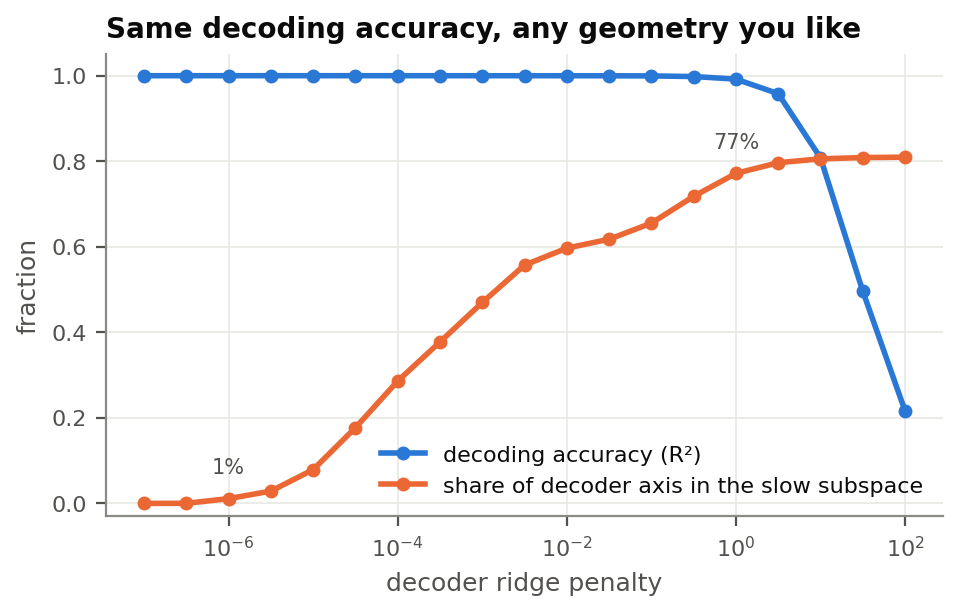
\includegraphics[width=0.55\linewidth]{fig2.png}
  \caption{Same decoding accuracy, very different direction. Blue: decoder $R^2$ against the ridge penalty. Orange: fraction of the decoder's weight vector inside the slow subspace.}
  \label{fig:decoder}
\end{figure}

\subsection{On the teacher, one well aimed channel is enough}\label{sec:res-teacher-steer}

As a positive control, while the plan loads the teacher's plan input has 25\% of full authority, 24 times random, and an LQR using it removes 69\% of the error (random 8\%, best single channel 89\%; \cref{fig:teacher-steer}a, open symbols). During the delay the best single channel has 100\% of full authority (\cref{fig:teacher-steer}b), since only one direction matters for the held plan, while random channels follow $k/N$. The teacher's own inputs are poorly aimed during the hold: the plan input has 10\%, the go input about 7\%, and both together 15\% of full authority, which still removes 57\% of the error at the fair setting. The linear analysis holds to within 10\% for requested pull changes up to about 0.1 (\cref{fig:teacher-steer}c).

The best push is the left eigenvector of the slow mode (agreement $0.2^\circ$), $24^\circ$ from the line of states, and the left and right slow eigenvectors are $39^\circ$ apart (\cref{fig:teacher-steer}d). The teacher is non-normal: a push tilted off the line loses a fast-decaying component that first feeds into the line (\cref{fig:nonnormal}, \cref{app:nonnormal}). A channel aimed exactly along the line gets $\cos^2 24^\circ = 0.83$ of the best authority.

\begin{figure}[t]
  \centering
  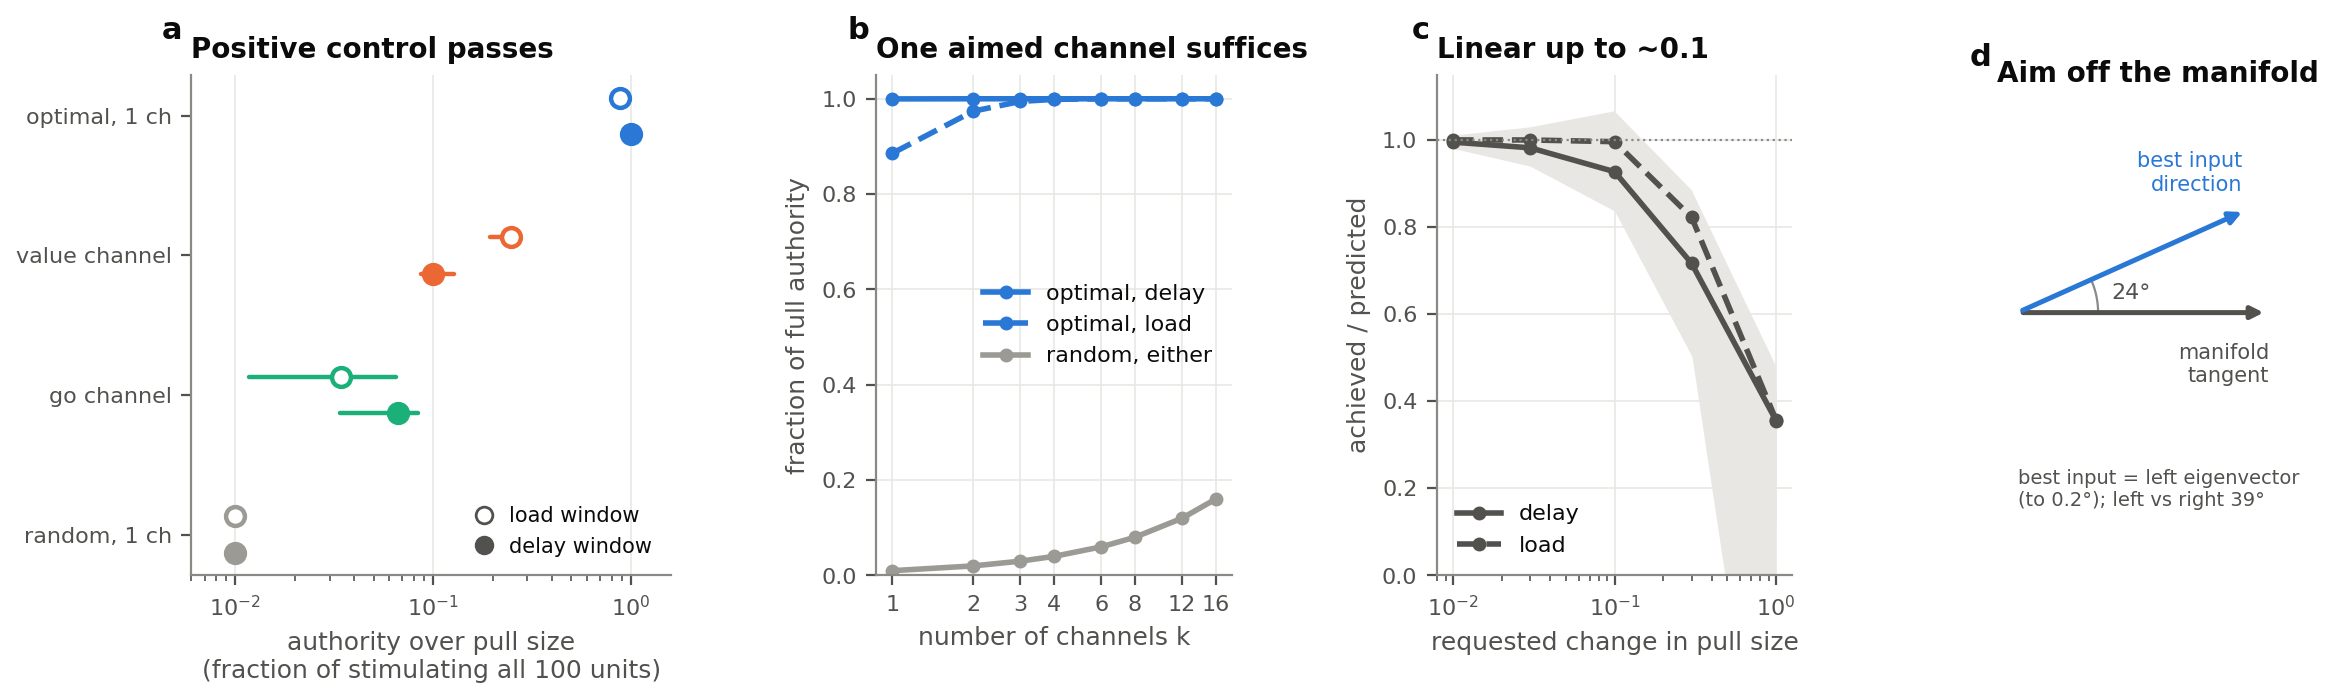
\includegraphics[width=\linewidth]{fig3.png}
  \caption{Steering the teacher. (a) Fraction of full authority for the best single channel, the plan input, the go input and one random channel, while the plan loads (open) and during the delay (filled); bars show the interquartile range over trials. (b) Best and random authority against the number of channels. (c) Achieved over predicted change against the requested change. (d) Angle between the best input direction and the line of states.}
  \label{fig:teacher-steer}
\end{figure}

\begin{figure}[t]
  \centering
  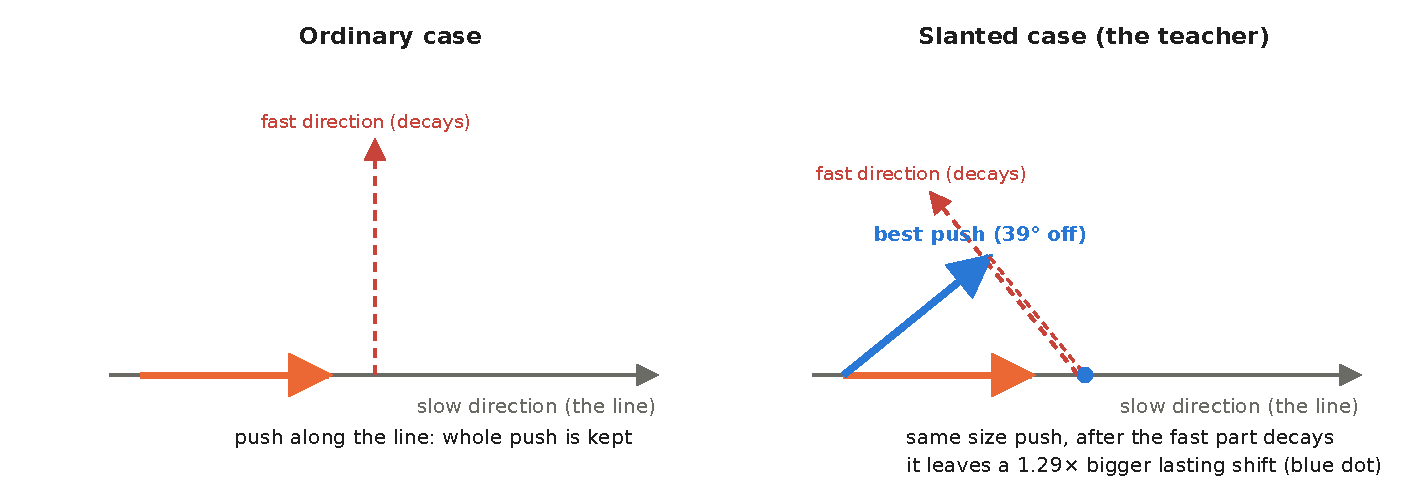
\includegraphics[width=0.72\linewidth]{d9_nonnormal.pdf}
  \caption{Why the best push is off the line. When the fast-decaying direction is slanted, a push tilted away from the line loses its fast part but leaves a larger lasting shift along the line (1.29 times for the teacher's $39^\circ$).}
  \label{fig:nonnormal}
\end{figure}

\subsection{Fitting the student: penalty, channels and generalisation}\label{sec:res-fit}

A stronger penalty lowers the fit to the recorded neurons (0.72 to 0.62 bits per spike from $\lambda=10^{-4}$ to 1) but improves held-out prediction (0.246 to 0.281); at $\lambda=10$ both collapse (0.20 and 0.10; \cref{fig:fit}a,b). More channels do the opposite: at $\lambda=0.01$, $k=16$ fits the recorded neurons best (1.15) and predicts held-out neurons worst (0.17), against 0.40 and 0.32 for $k=1$. The fit to the recorded neurons exceeds the 0.36 bits per spike of the teacher's true rates, which is only possible by fitting noise as input. A model chosen for the best fit to recorded neurons is therefore likely to over-use its controller.

Autonomy, the SURF selection criterion (how much of the activity the generator reproduces with the controller switched off), rises from $-0.54$ to about 0.05 as $\lambda$ increases to 1 (\cref{fig:fit}c). At all of these penalties the swap test (\cref{sec:res-plan}) shows that the pull is set by the controller (own share 0.01--0.05). With a strong penalty the controller concentrates its effort at the go cue, where its activity is 1.55 times its usual level (\cref{fig:fit}d).

\begin{figure}[t]
  \centering
  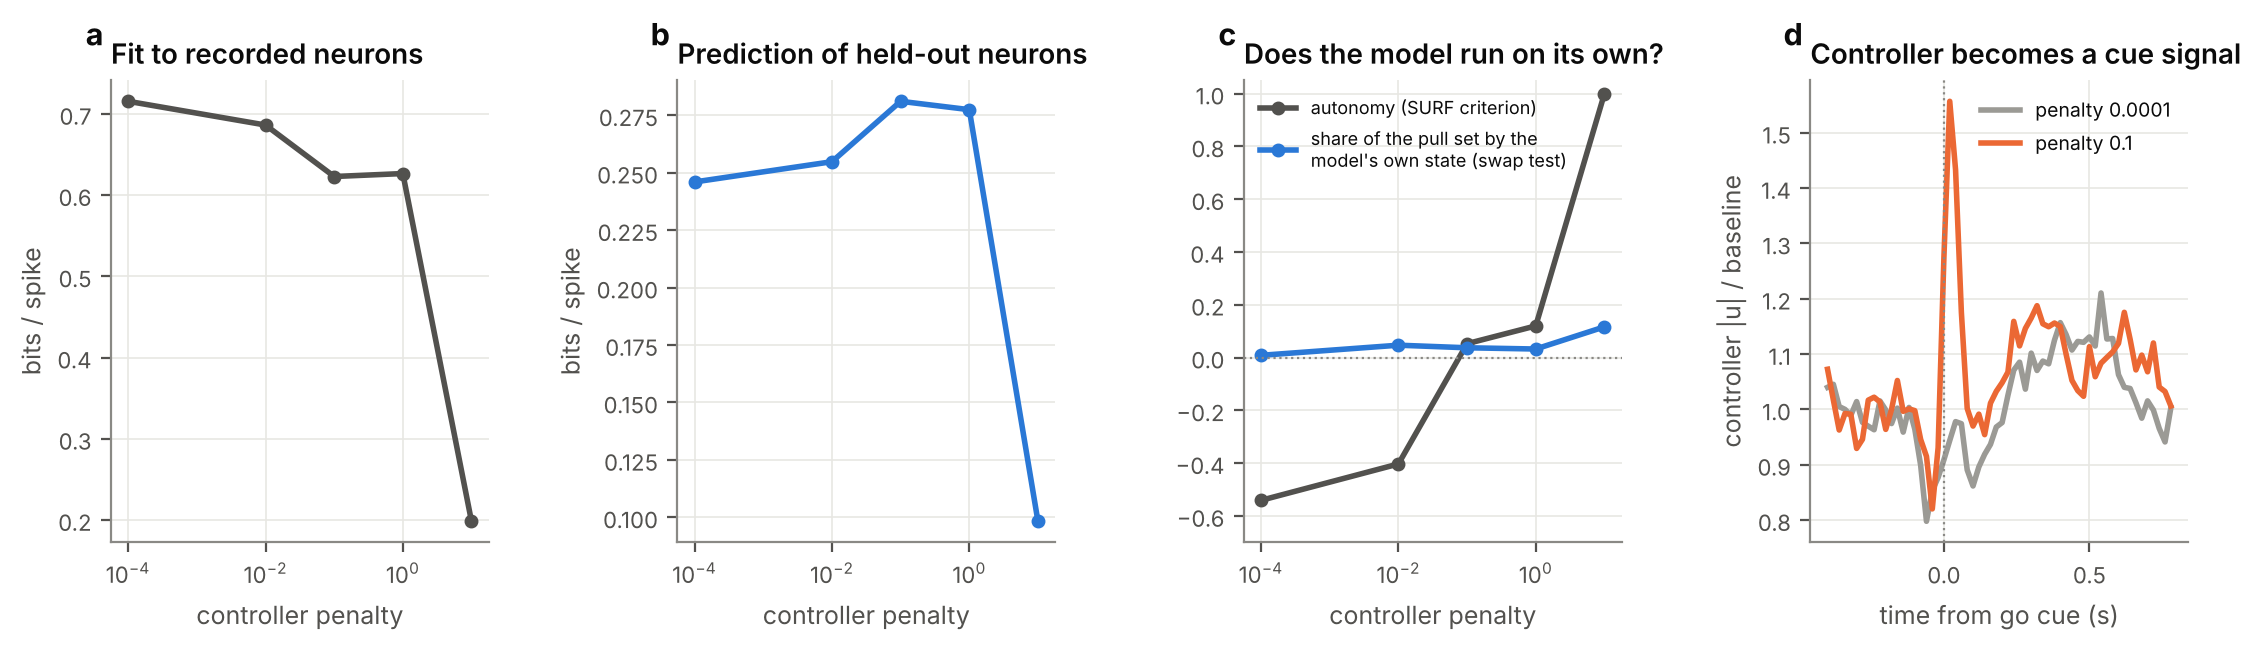
\includegraphics[width=\linewidth]{fig4.png}
  \caption{Free students with $k=4$ (seed 0) against the controller penalty. (a) Fit to the recorded neurons. (b) Prediction of held-out neurons. (c) Autonomy (the SURF criterion) and the swap-test share of the pull set by the model's own state. (d) Controller activity around the go cue relative to its usual level, at a low and a high penalty.}
  \label{fig:fit}
\end{figure}

\subsection{Inferred channels are poorly and inconsistently aimed}\label{sec:res-aim}

With $k=4$, over five seeds at each of $\lambda=10^{-4}$ and $0.1$, the inferred channels have 15--51\% of full authority during the delay (mean 32\%), against 6\% for random and 56--100\% for the best four channels of the same student (\cref{fig:aim}). A stronger penalty improves the best four (mean 59\% to 97\%) but not the inferred channels (30\% to 33\%), so the gap is largest for the cleanest models. One student ($k=8$, $\lambda=0.01$) was worse than random (8\% against 12.5\%).

The random seed matters as much as any setting (\cref{fig:seeds}). At $\lambda=0.1$ the five seeds give 15, 22, 51, 33 and 45\%, while the best four are at 93--100\% every time; at $\lambda=10^{-4}$ they give 24, 22, 42, 28 and 33\%. Autonomy is equally unstable (three fits near 0.05, two near 0.99). Held-out prediction does not identify the well aimed fits: the best predictor (0.291 bits per spike) has 33\% aim, and the two best aimed fits (51\% and 45\%) predict worst (0.258 and 0.226).

Refitting $k=1,2,4,8,16$ at $\lambda=0.1$ with three seeds each (\cref{fig:kseeds}; one $k=8$ fit diverged), the best $k$ channels reach 85\% at $k=1$ and 96--100\% from $k=4$, while the inferred channels average 65, 43, 29, 35 and 38\%. Adding channels does not bring them closer to the best, the spread between seeds is large at every $k$ (14, 40 and 61\% at $k=16$), and held-out prediction is best at $k=4$ (0.27) and worst at $k=16$ (0.16). While the plan loads, the students' channels range from 7\% (random level) to 51\%, against 25\% for the teacher's plan input.

\begin{figure}[t]
  \centering
  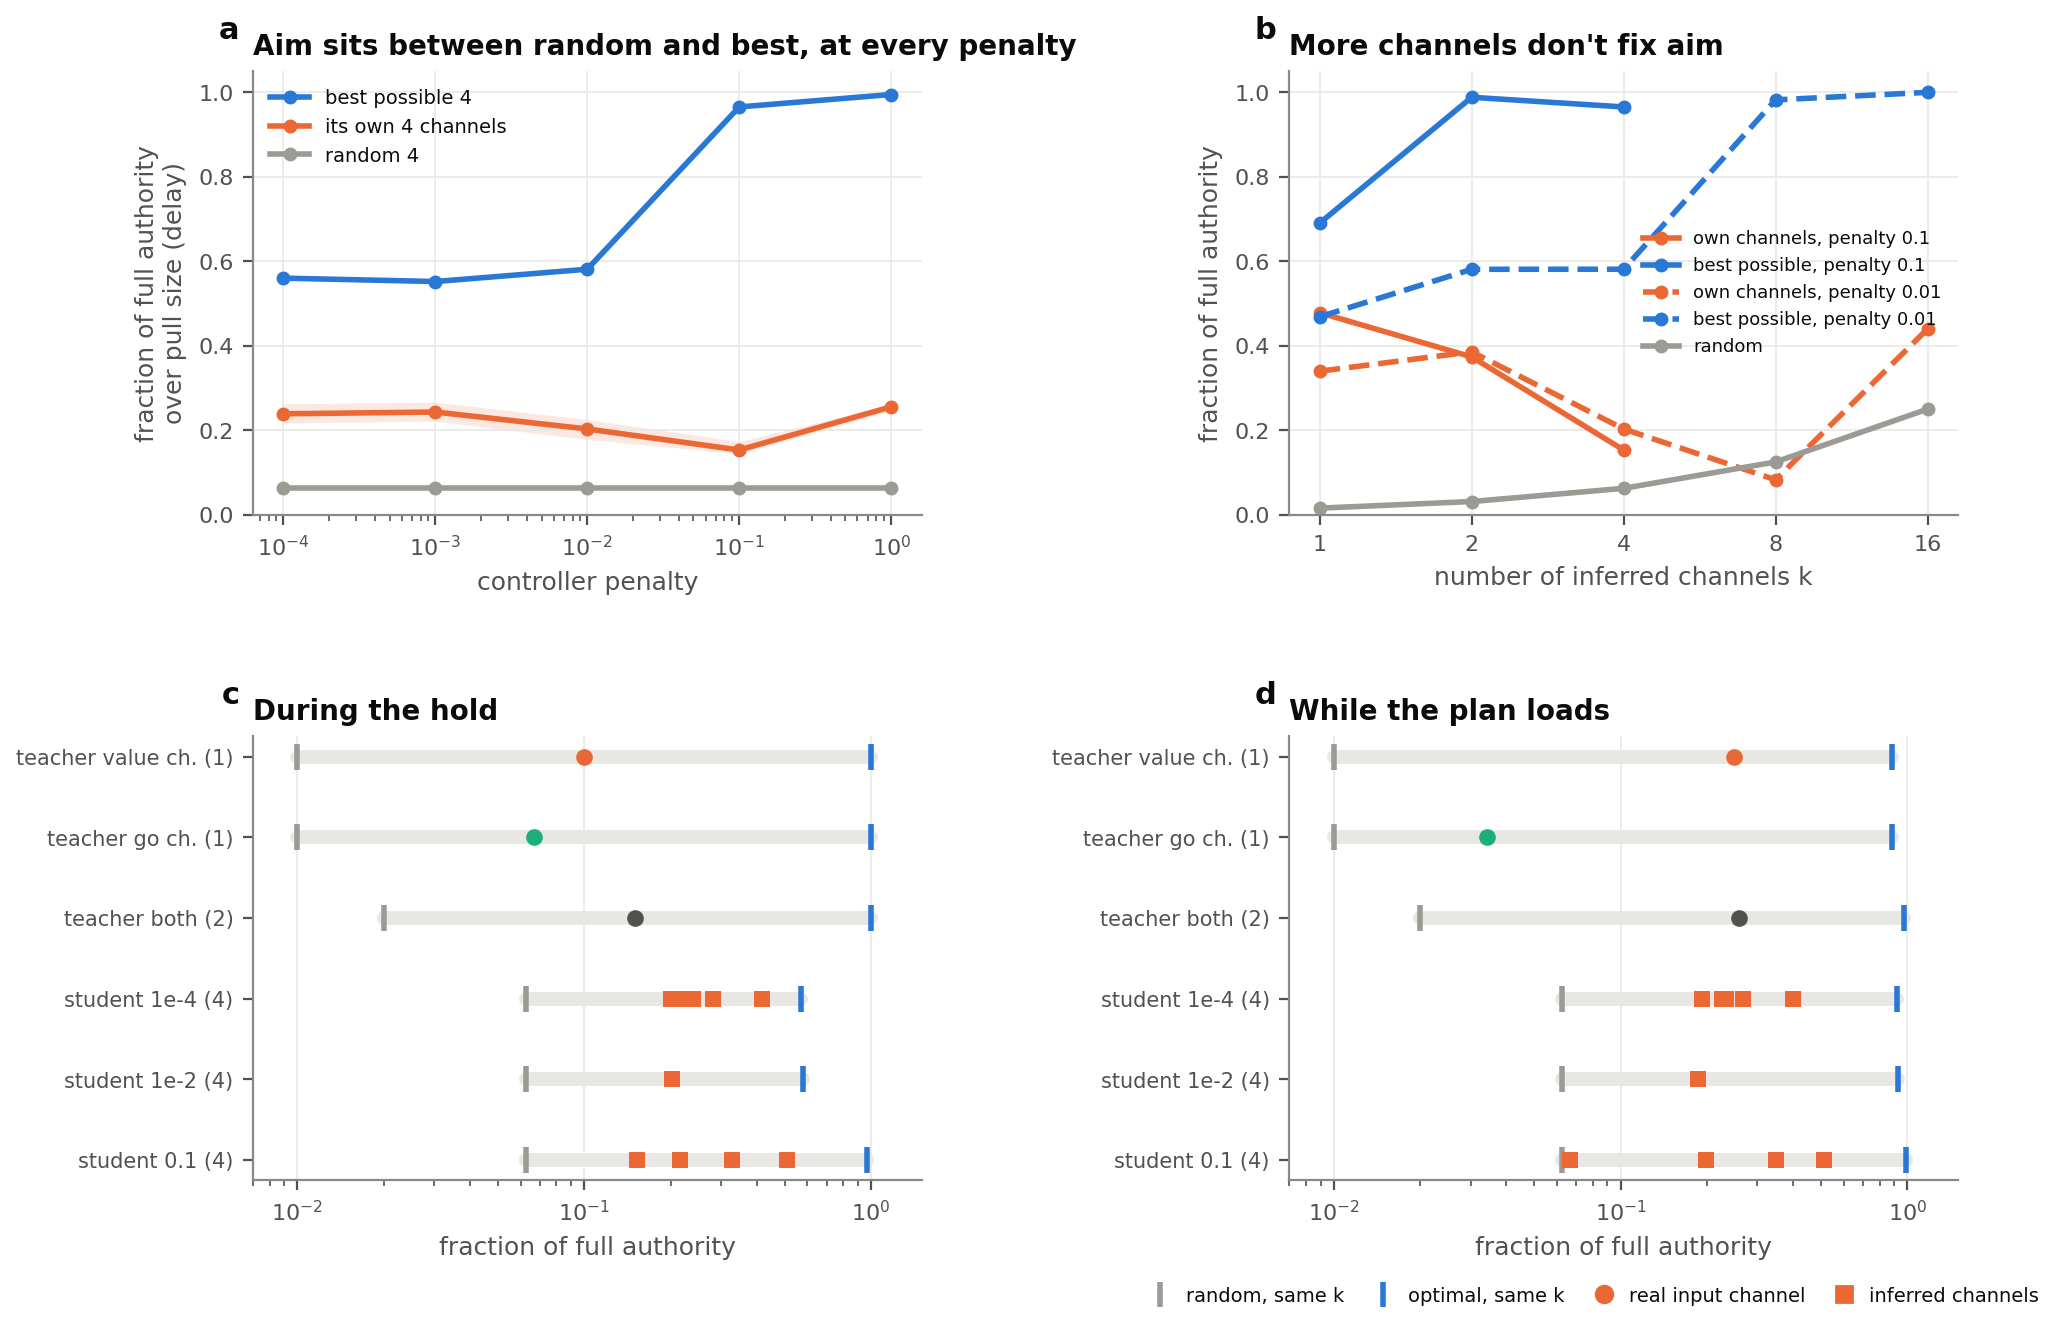
\includegraphics[width=\linewidth]{fig5.png}
  \caption{Steering through the students' inferred channels. (a) Fraction of full authority during the delay against the penalty (seed 0) for the student's own four channels (shading: spread over trials), the best four and random four. (b) Against the number of channels at two penalties. (c, d) Every channel set during the hold and while the plan loads; grey tick: random of the same size; blue tick: best of the same size; marker: the set tested. Each student appears once per seed.}
  \label{fig:aim}
\end{figure}

\begin{figure}[t]
  \centering
  \begin{subfigure}{0.49\linewidth}\centering
    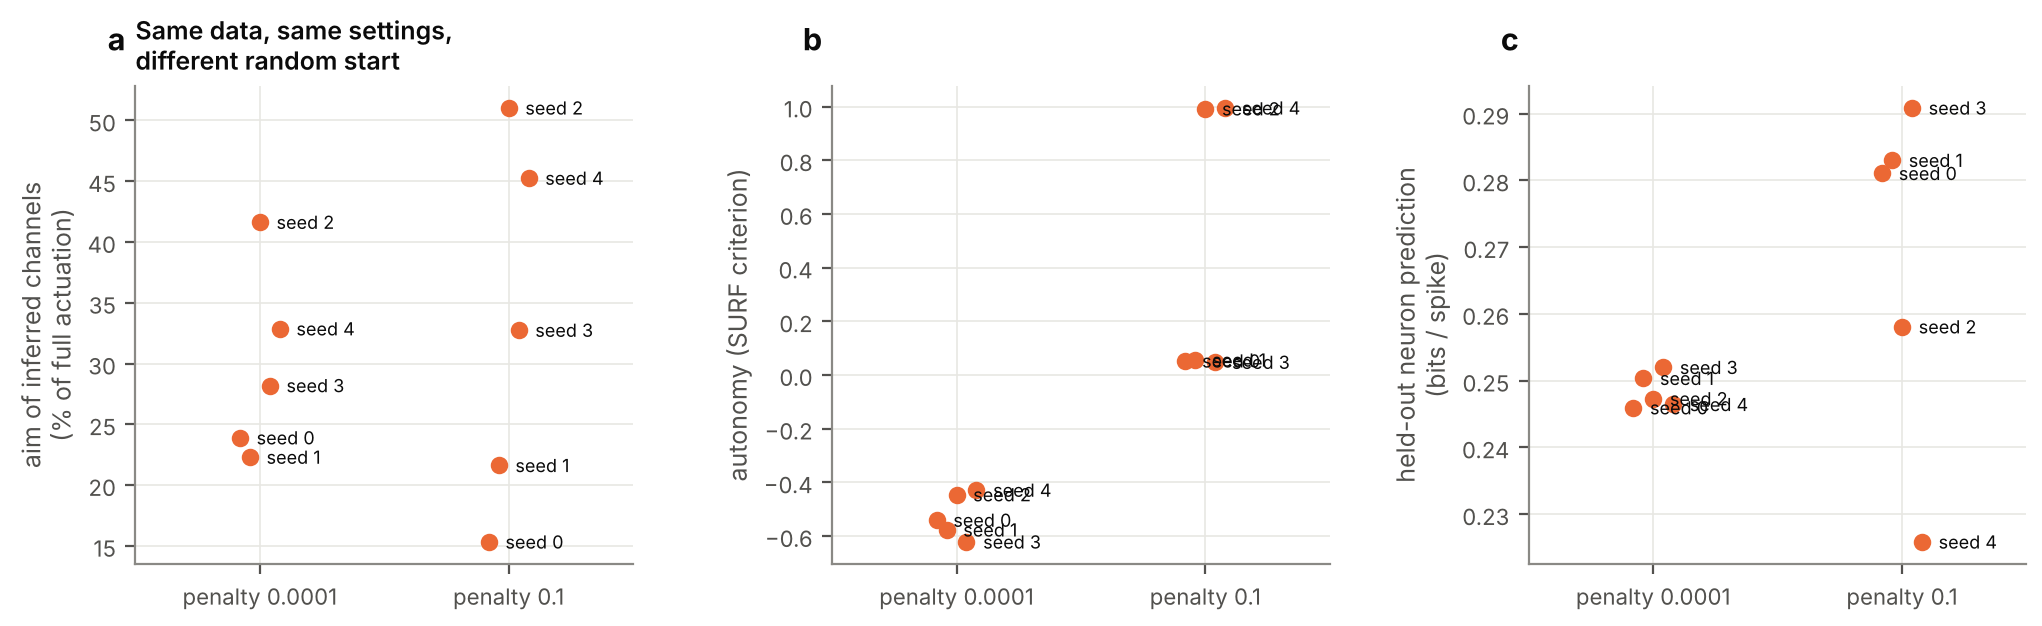
\includegraphics[width=\linewidth]{fig7.png}
    \caption{Five seeds, same data and settings.}\label{fig:seeds}
  \end{subfigure}\hfill
  \begin{subfigure}{0.49\linewidth}\centering
    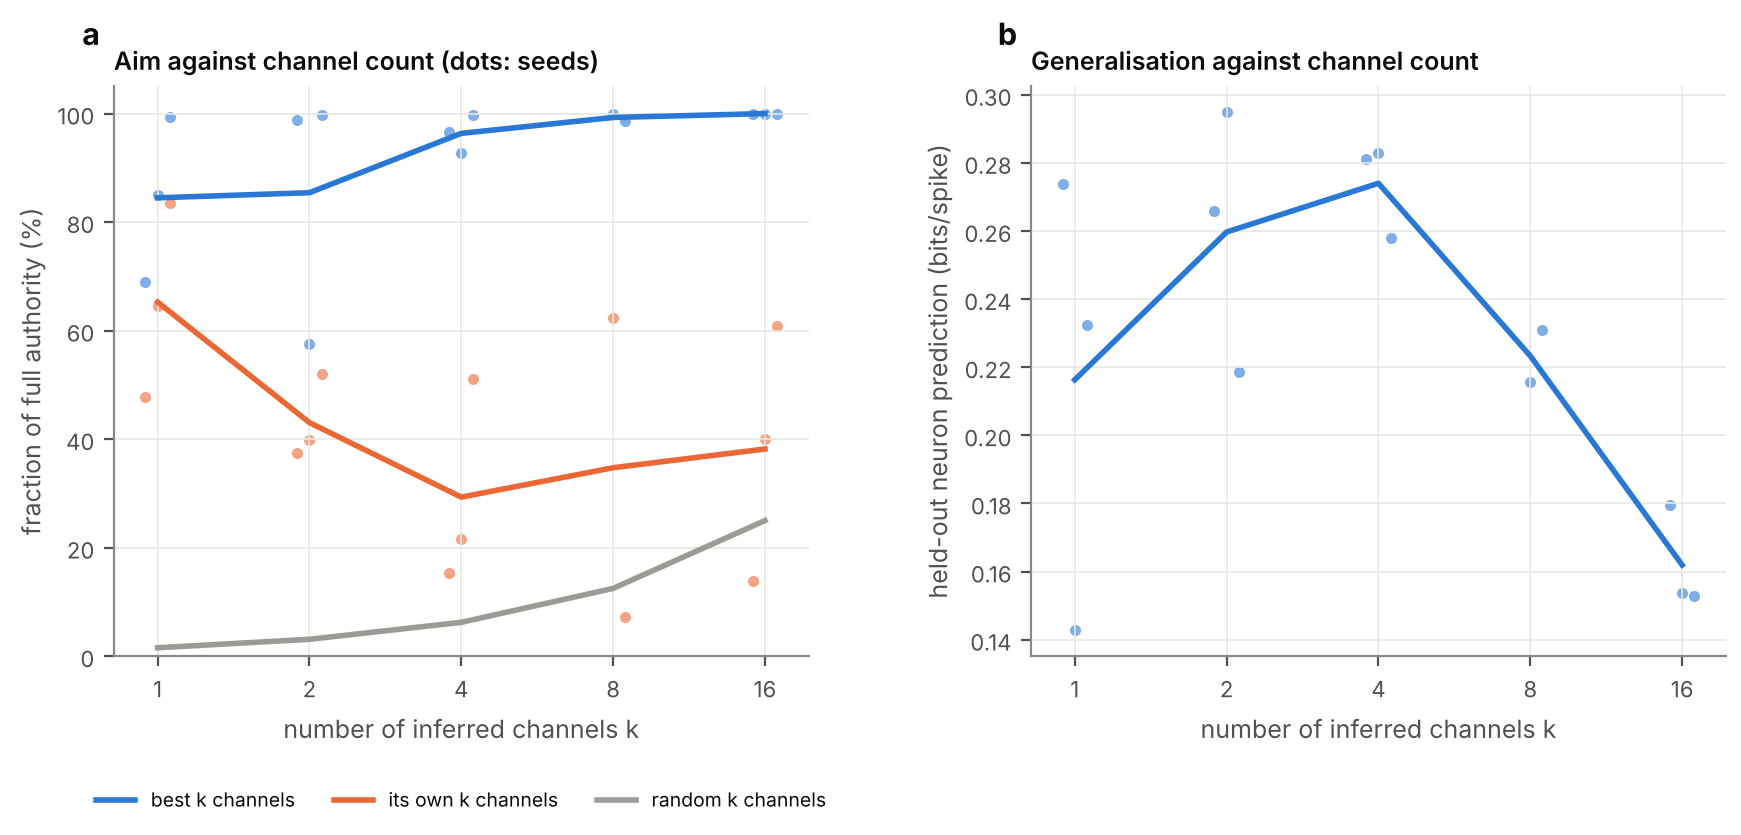
\includegraphics[width=\linewidth]{fig9.png}
    \caption{Number of channels at $\lambda=0.1$.}\label{fig:kseeds}
  \end{subfigure}
  \caption{Seed and channel-number dependence. (a) Aim of the inferred channels, autonomy and held-out prediction for five seeds at two penalties (numbers are seeds). (b) Fraction of full authority for the best $k$, the model's own $k$ and random $k$ channels (dots: single fits, lines: means), and held-out prediction.}
  \label{fig:seedsk}
\end{figure}

\subsection{Goal and effort cost}\label{sec:res-goal}

The SURF report described the channels as having negligible authority over ``a 128-dimensional state'', which suggests the LQR target was the full model state. The two goals differ greatly (\cref{fig:a-goals}). On the teacher, the whole-state goal cannot distinguish good aim from bad: real, random and best-for-behaviour channels all remove 13--14\% of the whole-state error, against 57\%, 14\% and 90\% for the behaviour goal (\cref{fig:goal}a). On students, random channels already remove 53--57\% of the whole-state error and inferred channels 62--66\%, while the behaviour goal separates the sets more clearly.

Sweeping the effort cost (\cref{fig:goal}b), the behaviour goal falls to 0.1\% only when $\rho$ is raised about 300 times above the fair value for random channels, 1800 times for the real inputs and 10\,000 times for the best four. The whole-state curves are nearly flat and stay above 1\% up to $10^5$ times. On the teacher, therefore, 0.1\% requires an effort cost hundreds to thousands of times above the range in which the controller is useful. One way this can happen unintentionally is a cost set in absolute units while the inferred channels enter the generator with a small effect.

\begin{figure}[t]
  \centering
  \begin{subfigure}{0.49\linewidth}\centering
    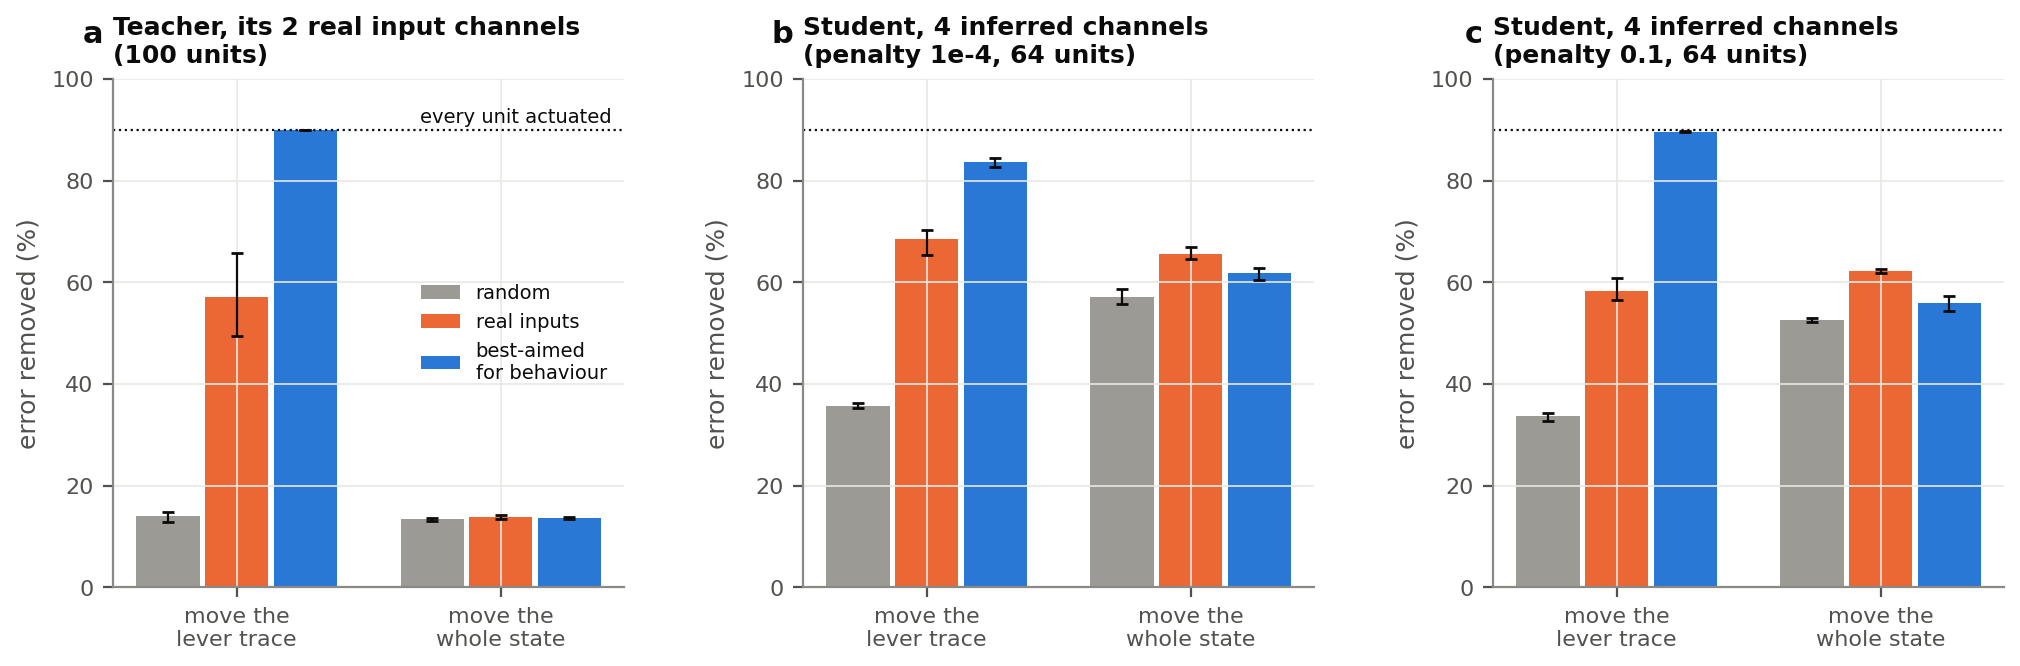
\includegraphics[width=\linewidth]{fig6.png}
    \caption{Behaviour goal versus whole-state goal.}
  \end{subfigure}\hfill
  \begin{subfigure}{0.49\linewidth}\centering
    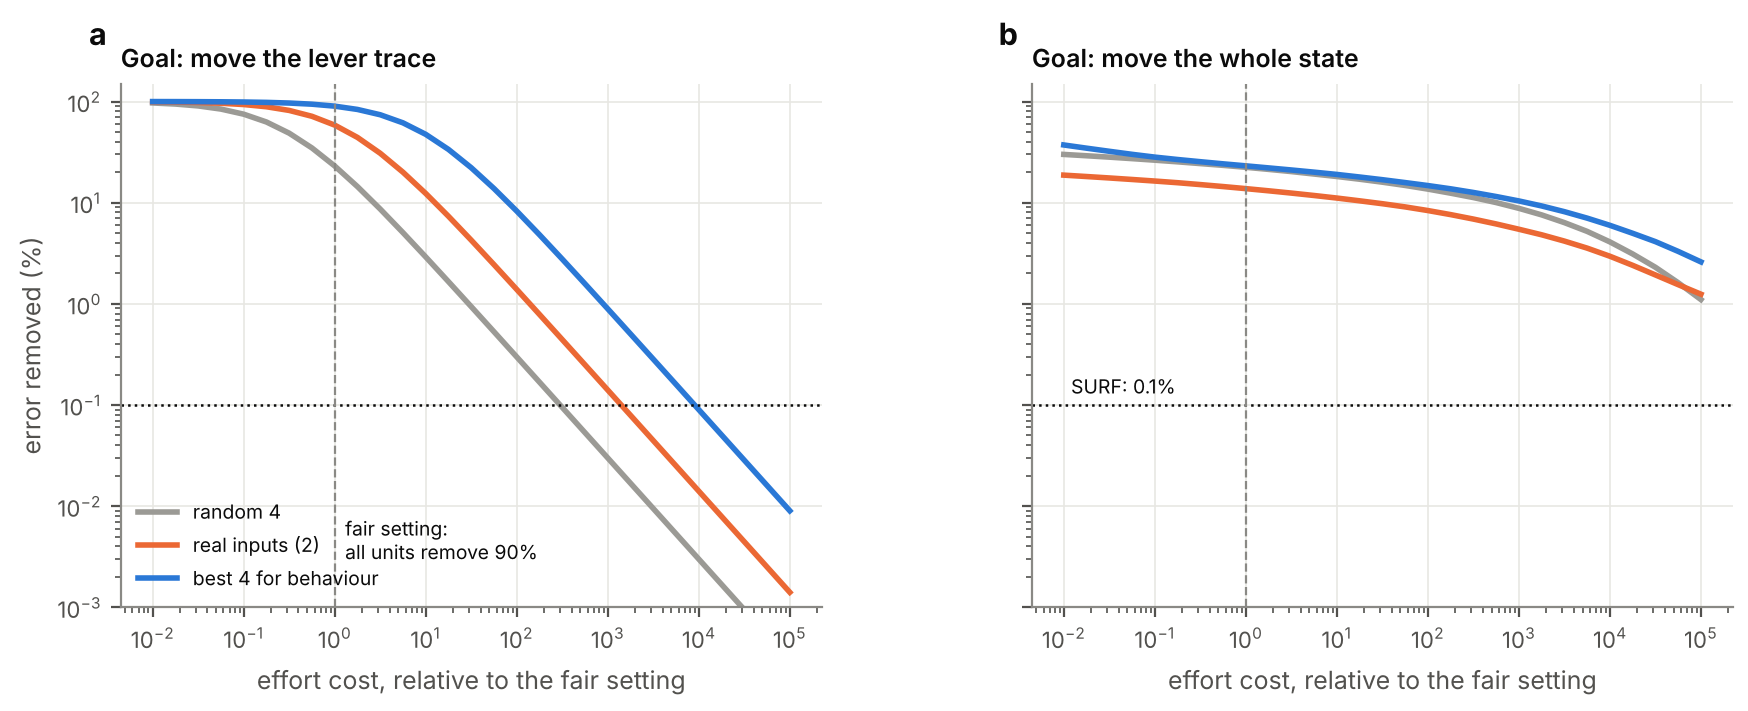
\includegraphics[width=\linewidth]{fig8.png}
    \caption{Error removed against effort cost.}
  \end{subfigure}
  \caption{(a) Error removed for random channels, the channels tested and the channels best aimed for behaviour, when the goal is the lever trace or the whole state (dotted line: full actuation, 90\% by construction; bars: spread over 64 trials). (b) Error removed on the teacher against the effort cost relative to the fair setting (dashed), for both goals, log axes; dotted line: the SURF value of 0.1\%. Medians over 48 trials.}
  \label{fig:goal}
\end{figure}

\subsection{Replication on an independently trained teacher}\label{sec:res-rep}

\Cref{tab:rep} repeats the main measurements on teacher A2 with a new spike dataset and three student seeds per penalty. All ground-truth findings and student findings repeat.

\begin{table}[t]
  \centering
  \caption{Replication on an independently trained teacher.}
  \label{tab:rep}
  \small
  \begin{tabularx}{\linewidth}{@{}Xll@{}}
    \toprule
    & Teacher A & Teacher A2 \\
    \midrule
    Lever $R^2$; pull--plan correlation & 0.999; 0.999 & 0.999; 0.999 \\
    Slow eigenvalue; next eigenvalue & 0.99; 0.64--0.70 & 0.99; 0.76 \\
    Best single channel, delay (fraction of full authority) & 100\% & 100\% \\
    Real inputs together, delay & 15\% & 10\% \\
    Plan input while the plan loads & 25\% & 21\% \\
    Best push vs.\ line of states & $24^\circ$ & $26^\circ$ \\
    Left vs.\ right slow eigenvector & $39^\circ$ & $42^\circ$ \\
    Student $\lambda=10^{-4}$: own 4 / best 4 / random 4 & 22--42 / 56--67 / 6\% & 15--34 / 58--62 / 6\% \\
    Student $\lambda=0.1$: own 4 / best 4 / random 4 & 15--51 / 93--100 / 6\% & 28--35 / 89--100 / 6\% \\
    Swap test, teacher: own share & 1.00 & 1.00 \\
    Shift test, teacher: gain & 0.81 & 0.82 \\
    Swap test, free students: own share & $-0.01$ to 0.06 & 0.08 to 0.27 \\
    Shift test, free students: gain & $-0.02$ to 0.15 & $-0.02$ to 0.01 \\
    \bottomrule
  \end{tabularx}
\end{table}

\subsection{Public monkey data}\label{sec:res-mc}

On MC\_Maze, the best single channel has 78--86\% of full authority over the reach and the best four 84--98\%, so a few well aimed channels suffice in a model of real motor cortex too (\cref{fig:mc}). The inferred channels are close to random: at $\lambda=10^{-4}$ the four channels have 4, 5 and 8\% against 6\% for random (0.7--1.3 times random), and at $\lambda=0.1$ they have 10--18\% (1.6--2.9 times random). Results are the same for pushes around the go cue. With 16 channels the inferred channels reach 53--61\%, but random 16 already have 25\% and the best 16 have 100\%, and these models predict held-out neurons worst (0.08 against 0.13--0.145 bits per spike for $k=4$). Changing the decoder ridge from $10^{-4}$ to $10^{-2}$ changes the aim by less than 3.5 percentage points in 8 of 10 fits.

The swap test on these models (giving each trial another trial's inferred inputs over the whole window) depends on the model's settings (\cref{fig:toldwhen}c). With one channel the reach follows the trial's own initial state (own share 0.77--0.88 for $x$, 0.71--0.81 for $y$); with 16 channels it follows the swapped-in inputs ($-0.03$ to $-0.01$); with four channels it lies in between and varies with penalty and seed (0.48--0.72 for $x$ at $\lambda=0.1$, 0.06--0.24 at $10^{-4}$). These models predict held-out neurons about equally well (0.11--0.145 bits per spike).

\begin{figure}[t]
  \centering
  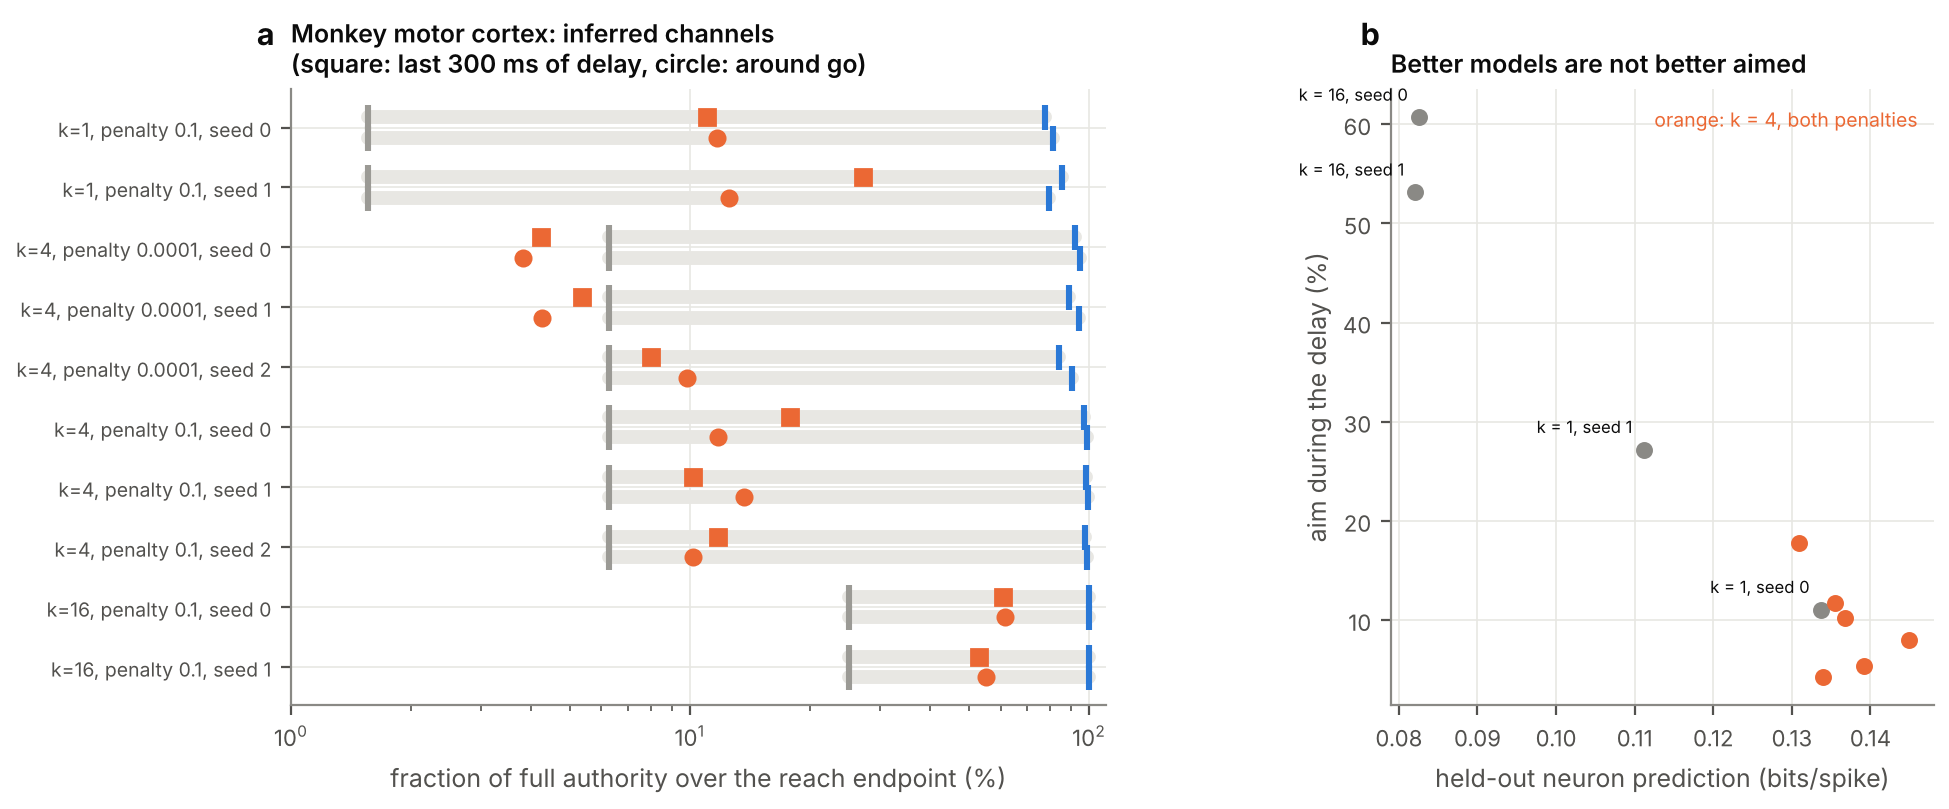
\includegraphics[width=\linewidth]{fig10.png}
  \caption{Monkey motor cortex (MC\_Maze, large session). (a) Fraction of full authority over the reach for each fit's own channels (orange), random channels of the same number (grey tick) and the best channels (blue tick); squares: pushes in the last 300\,ms of the delay, circles: around the go cue. (b) Aim during the delay against held-out prediction.}
  \label{fig:mc}
\end{figure}

\subsection{Where does the fitted model keep the plan?}\label{sec:res-plan}

The tests of \cref{sec:tests} separate the two teachers cleanly (\cref{fig:plan}, dashed lines). In teacher A the pull follows the trial's own plan after a swap (own share 1.00, partner 0.00), a shift along the line reaches the pull with gain 0.81, and exactly one direction persists over 20 steps (0.99 left, below 0.01 in every other direction). In teacher B the pull follows the swapped-in input (own share 0.00), a shift has no effect (gain 0.00) and nothing persists.

\begin{figure}[t]
  \centering
  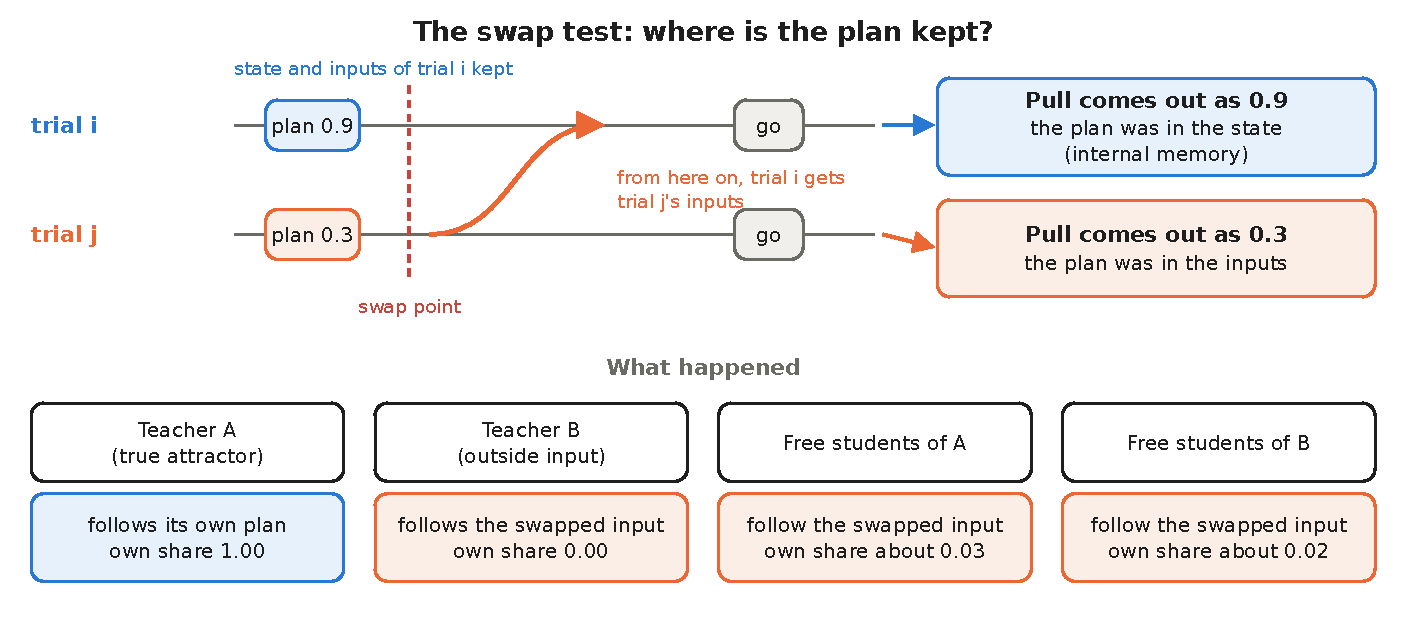
\includegraphics[width=0.9\linewidth]{d14_swap.pdf}
  \caption{The swap test. After the plan is loaded, a trial is given another trial's inputs. A system that holds the plan in its state pulls according to its own plan; one that is fed the plan follows the swapped-in inputs.}
  \label{fig:swap}
\end{figure}

The free students of teacher A do not hold the plan. At every penalty up to 1 (16 fits) the own share is $-0.01$ to 0.06 (median 0.03) and the partner share 0.91--1.03. Swapping only from 3 steps before the go cue, with the whole delay untouched, gives almost the same result in most fits, so the plan is not carried by the state at the go cue either; 51--69\% of the controller's power is spent at and after the go cue. A shift during the delay reaches the pull with gain 0.00 (range $-0.02$ to 0.15), against 0.81 in the teacher, and the largest real positive 20-step eigenvalue is 0.00--0.55 (median 0.31), against 0.99. Even at $\lambda=10$ the own share reaches only 0.04--0.12. The students reproduce the spikes by a different mechanism: the teacher remembers the plan, and the student is handed it again by its controller when the pull is made.

The students of teacher B give the same answers (own share $-0.05$ to 0.04 for 11 fits, shift gain $-0.02$ to 0.01). For teacher B this answer is correct, but the students of the two teachers are indistinguishable on every test, so the fitted model cannot reveal whether the circuit has a memory. Teacher A2 repeats the result (truth: own share 1.00, gain 0.82, one persistent direction at 0.97; six students: own share 0.08--0.27, gain $-0.02$ to 0.01).

\begin{figure}[t]
  \centering
  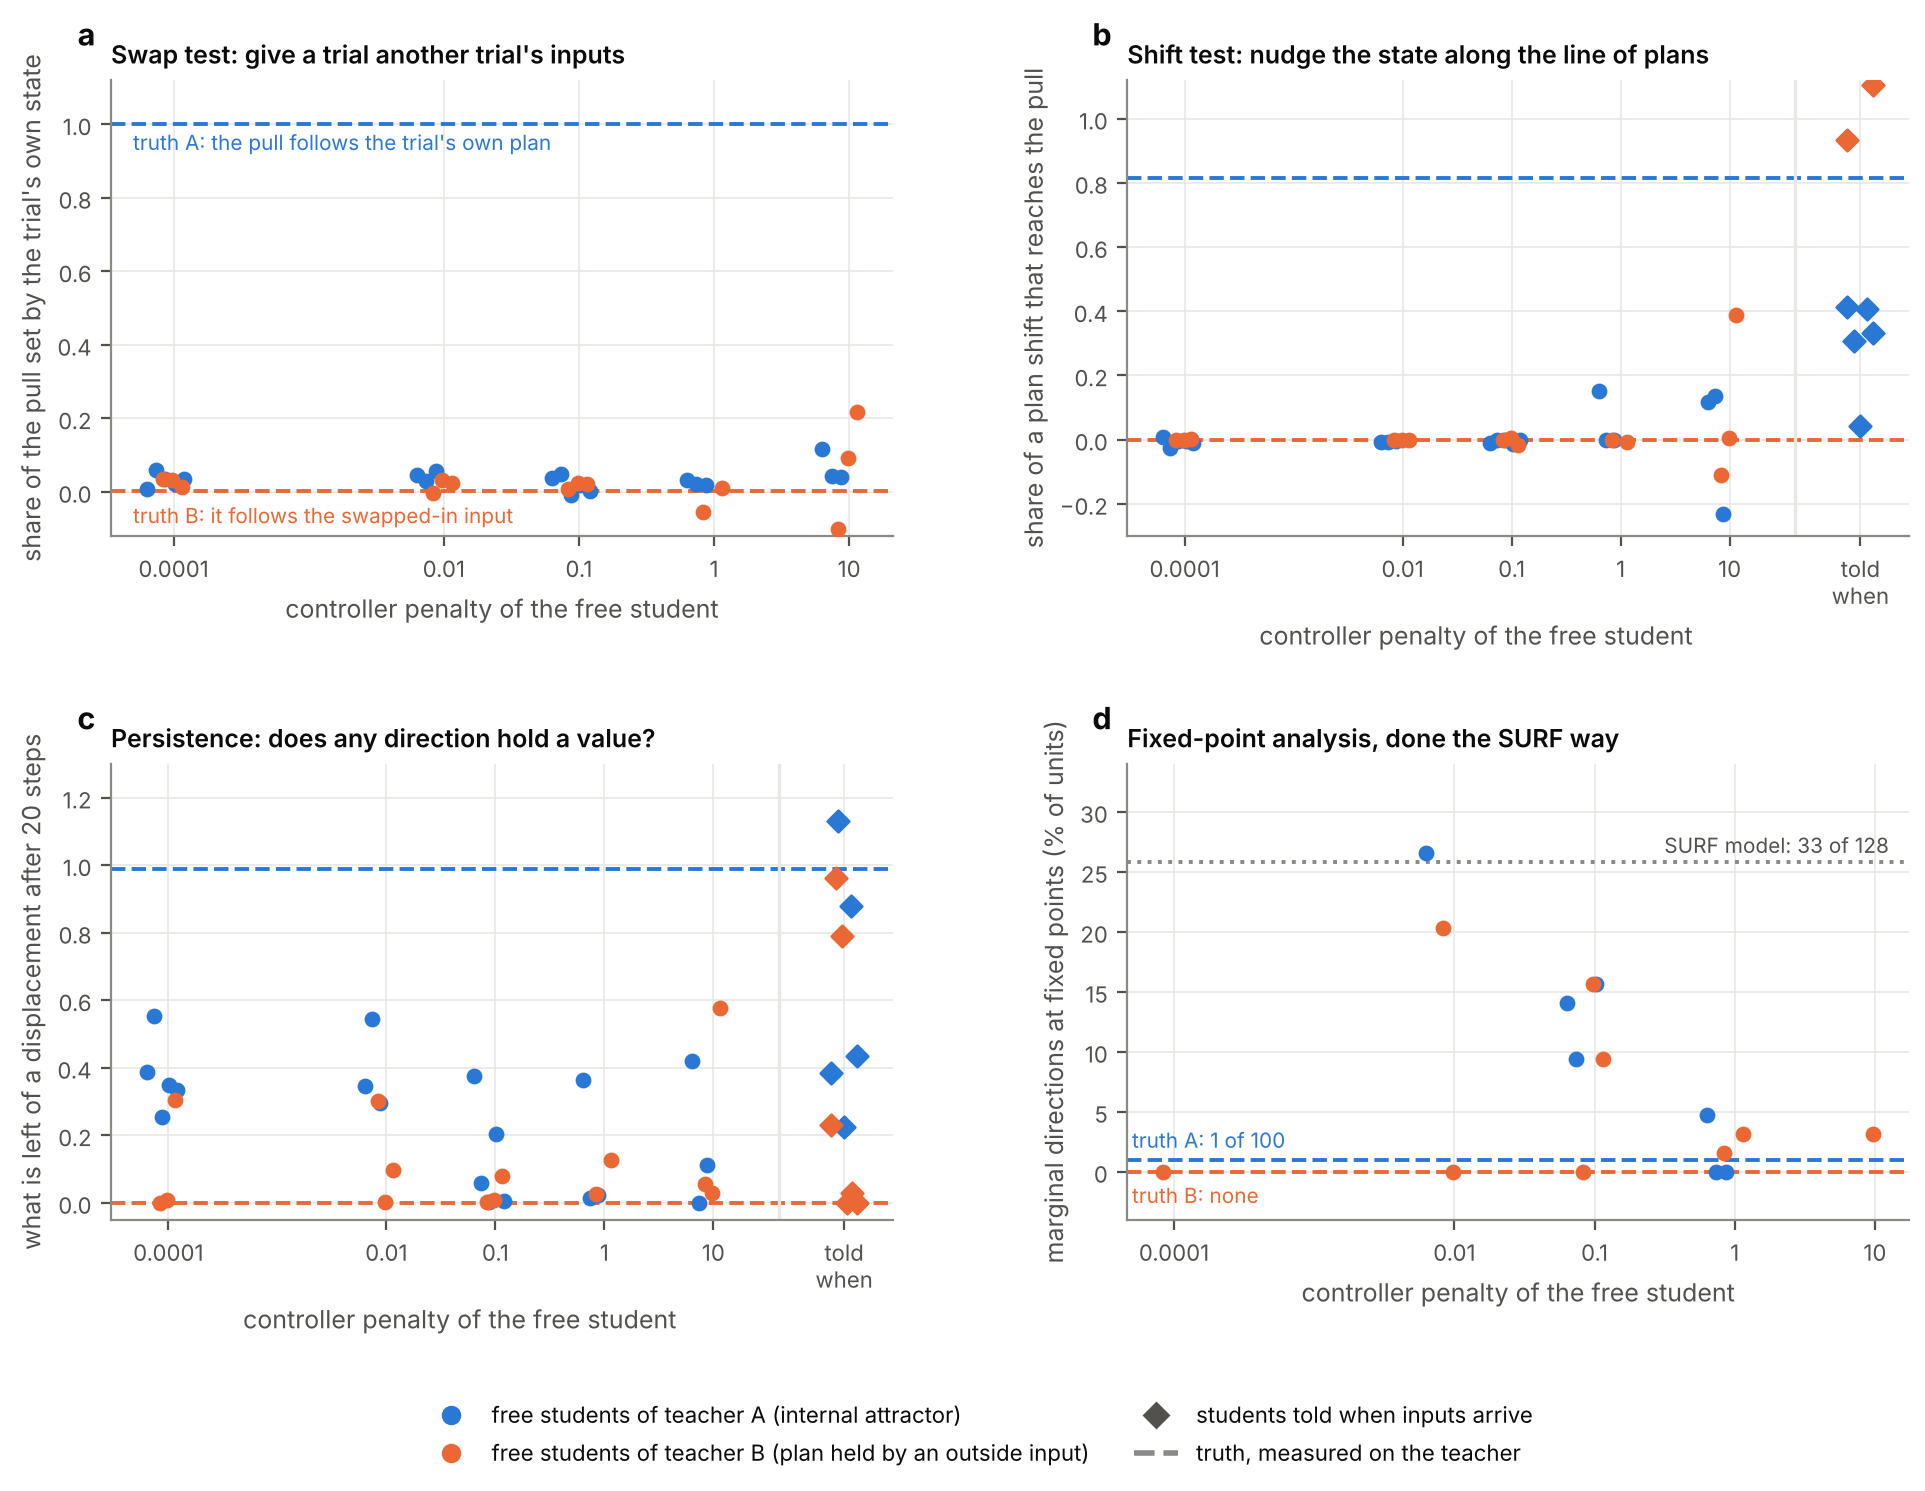
\includegraphics[width=\linewidth]{figP1_plan.png}
  \caption{Where is the plan kept? Free students of teacher A (blue) and teacher B (orange) against the penalty; dashed lines: truth on each teacher; diamonds: told-when students (\cref{sec:res-toldwhen}). (a) Swap test: share of the pull following the trial's own plan. (b) Shift test gain. (c) Largest real positive eigenvalue of the 20-step propagator. (d) Marginal directions at fixed points, as a percentage of the model's units (fits with at least 5 fixed points).}
  \label{fig:plan}
\end{figure}

\subsection{Marginal directions that the circuit does not have}\label{sec:res-marginal}

Teacher A has exactly one eigenvalue above 0.8 at its fixed points, along the line. In the free students of teacher A with at least five fixed points (7 of 19 fits), fixed-point analysis finds 0 to 17 marginal directions out of 64 and 3 to 39 eigenvalues above 0.8; at $\lambda\in\{0.01,0.1\}$ the marginal count is 6--17, i.e.\ 9--27\% of the units, the same range as the 26\% (33 of 128) of the SURF model (\cref{fig:plan}d). Students of teacher B, which has no slow direction, show 0 to 13. Many of these directions are complex or negative, and \cref{sec:res-plan} shows none carries the plan. They are better understood as directions the data never forced to decay: with 64 units and a rank-12 readout, displacements in most directions barely change the predicted spikes. A marginal count therefore cannot, on its own, establish an attractor in the circuit; it does not exclude one either.

\subsection{A student that is told when inputs arrive}\label{sec:res-toldwhen}

Because the free student never holds the plan, we fitted the told-when student (five seeds on teacher A, six on teacher B). On teacher A it predicts held-out neurons with 0.34--0.37 bits per spike, against 0.22--0.29 for the 16 free students and 0.40 for the teacher's true rates (\cref{fig:toldwhen}a). Its single-trial rates are also much closer to the truth ($R^2$ 0.87--0.95 against $-0.27$ to 0.38 for the free students; the free student's per-trial inputs fit spike noise). Its pull follows the plan ($r=0.92$--0.99) and it has exactly one persistent direction, the structure of the teacher, although the memory is leakier and seed-dependent (0.22 to 1.13 of a displacement left after 20 steps; shift gains 0.04 to 0.41, against 0.99 and 0.81 in the teacher).

On teacher B, which has no memory, the told-when students were harder to train. Two of the six carried the plan to the pull ($r=0.65$ and 0.99), and both did it by building a slow direction that holds the plan (0.79 and 0.96 of a displacement left after 20 steps, truth 0.00), so a shift reaches the pull with gain about 1 (truth 0.00). The other four did not carry the plan ($r$ between $-0.07$ and 0.15), and three of them also fitted poorly (held-out 0.15--0.24). The fit that predicts held-out neurons best among all models of teacher B (0.31 bits per spike, against 0.09--0.25 for the free students) is the one with the most complete invented memory. So no told-when fit of teacher B found the true mechanism: it either invented a memory or failed.

\Cref{fig:grid} summarises the $2\times2$ result. The free student reports a plan supplied by inputs on both teachers. The told-when student reports an internal memory on teacher A, and on teacher B in both fits that carried the plan. Each is right on one teacher and wrong on the other. The best held-out prediction on each teacher comes from a told-when fit, including on teacher B, where its mechanism is wrong. What separates the two circuits is a perturbation: swapping or silencing the input, or shifting the state and watching whether the shift lasts.

\begin{figure}[t]
  \centering
  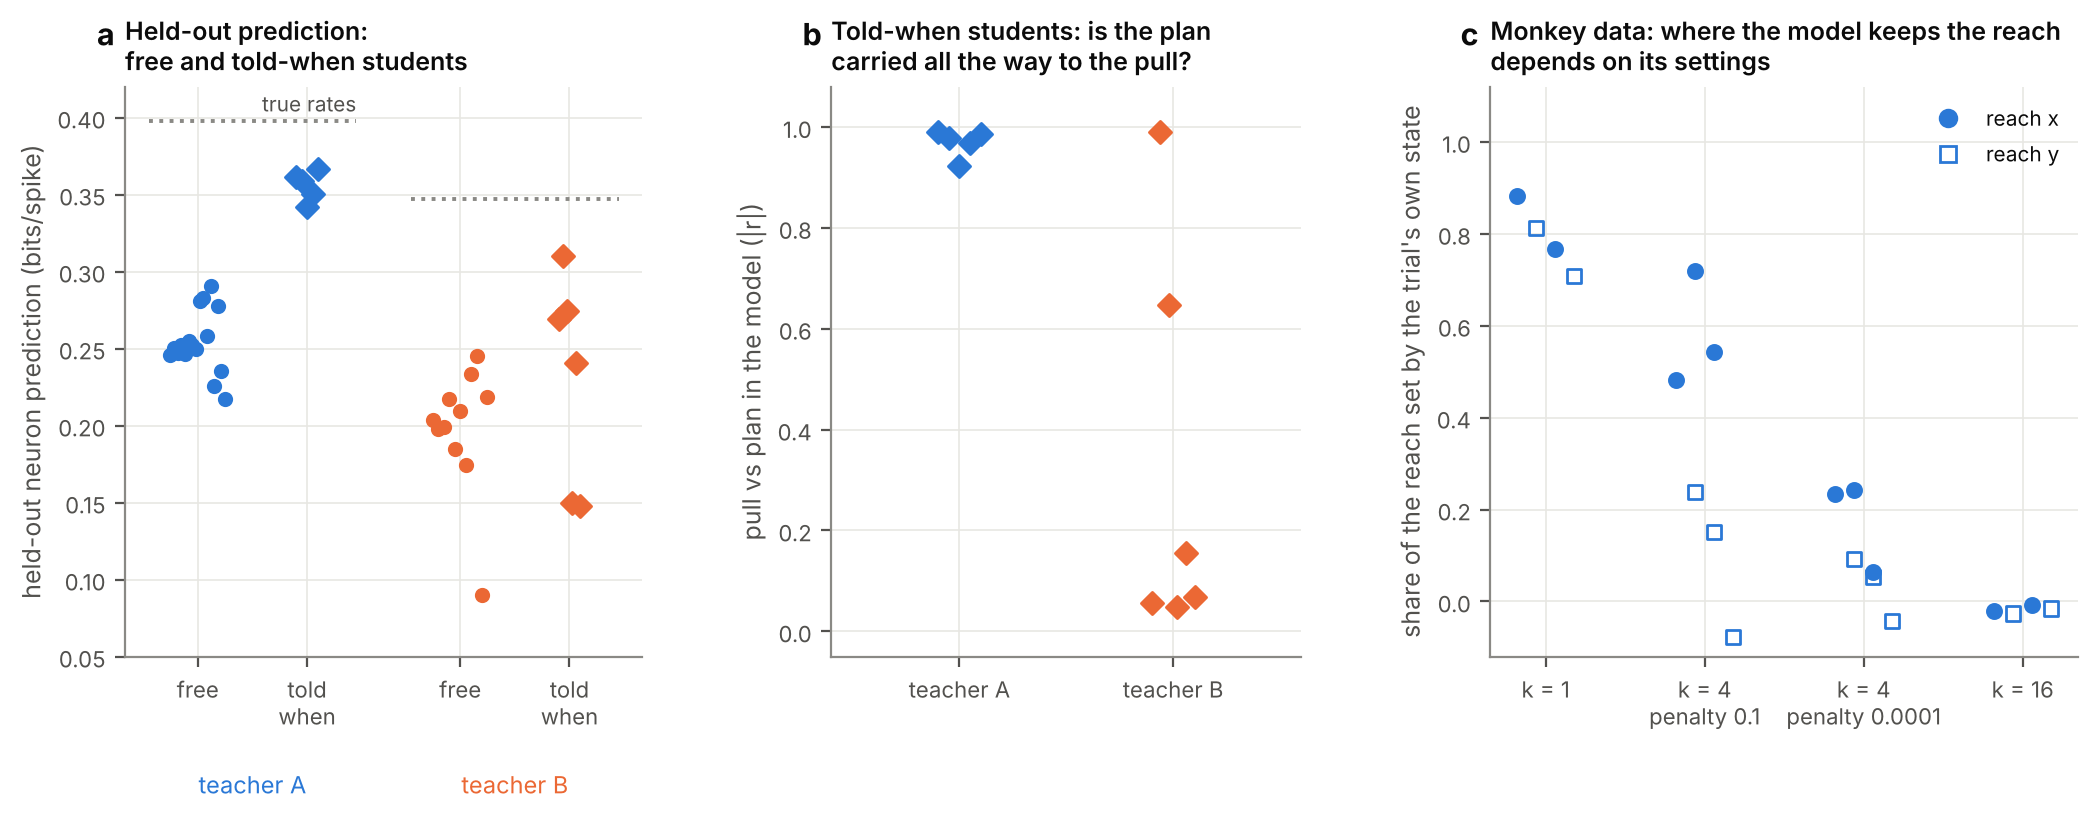
\includegraphics[width=\linewidth]{figP2_event_mc.png}
  \caption{(a) Held-out prediction by free students (dots, $\lambda\le1$) and told-when students (diamonds) on both teachers; dotted lines: the teacher's true rates. (b) How well the pull follows the plan in the told-when students. (c) MC\_Maze: share of the reach following the trial's own state under the swap test, for models with 1, 4 and 16 channels.}
  \label{fig:toldwhen}
\end{figure}

\begin{figure}[t]
  \centering
  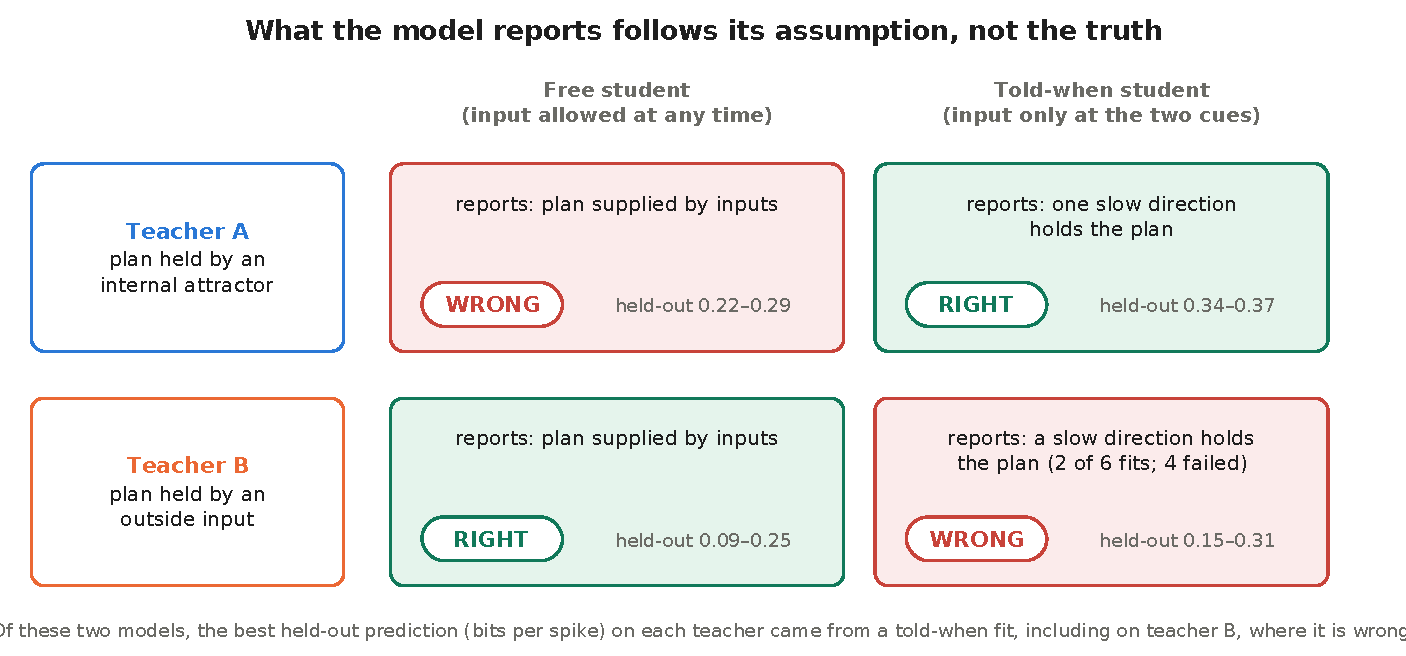
\includegraphics[width=0.85\linewidth]{d15_grid.pdf}
  \caption{Two circuits and two model assumptions. The mechanism the fitted model reports follows its assumption, and held-out prediction does not reveal which assumption is right.}
  \label{fig:grid}
\end{figure}

\subsection{Does the model tell us where to push the circuit?}\label{sec:res-transfer}

Translated to the teacher through the recorded neurons (\cref{sec:transfer}), the free students' estimate of the teacher's sensitivity is unrelated to the truth: its median cosine with $\vect s_T$ is $-0.22$ to 0.32 across the 16 fits, the sign is right about as often as wrong, and a push along it reaches $-6$\% to 10\% of full authority (negative means the pull moves the wrong way). For the five told-when students of teacher A the sign is right in 79--94\% of time steps, but the direction is still far off (cosine 0.07--0.15) and the push reaches 1--3\%, against the 87\% ceiling.

We think the reason is general. The best push is the left eigenvector of the slow mode, which is set by how the circuit relaxes after a displacement off the line of states. Noise-free recordings contain only states on the line, so nothing in the data constrains the dynamics off it: the right eigenvector can be learned from recordings and the left one cannot. Trial-to-trial fluctuations in real circuits do visit states off the line, which is the idea behind residual dynamics \citep{galgali2023}. The translation used here (matching the immediate effect on recorded neurons) is one of several possible, so this result is preliminary.

\subsection{Full LFADS fits the recordings much better}\label{sec:res-lfads-fit}

Full LFADS fits the recordings far better than the free student (\cref{fig:lfads}a). On held-out trials of teacher A its single-trial rates match the true rates with $R^2=0.94$--0.96 (at \kl{} $10^{-5}$ and $10^{-4}$), against $-0.27$ to 0.38 for the free students and 0.87--0.95 for the told-when students. It predicts held-out neurons with 0.36--0.37 bits per spike (true rates 0.40), and its pull follows the plan ($r=0.99$) on trials it was not trained on. At \kl{} $=10^{-4}$, the SURF cfg06 value, the controller is almost unused: the generator alone reproduces 94--97\% of the activity, as in the SURF model (97\% and 87\% in the two mice; \cref{fig:lfads}f). At $10^{-5}$ the controller is used, mostly at and after the go cue (70--82\% of its power). Three seeds at $10^{-4}$ agree closely with each other: on held-out trials the generator state of one fit predicts that of another with cross-validated $R^2=0.97$, against 0.15--0.35 for the free students, while their controller outputs agree much less ($R^2=0.43$).


\begin{figure}[t]
  \centering
  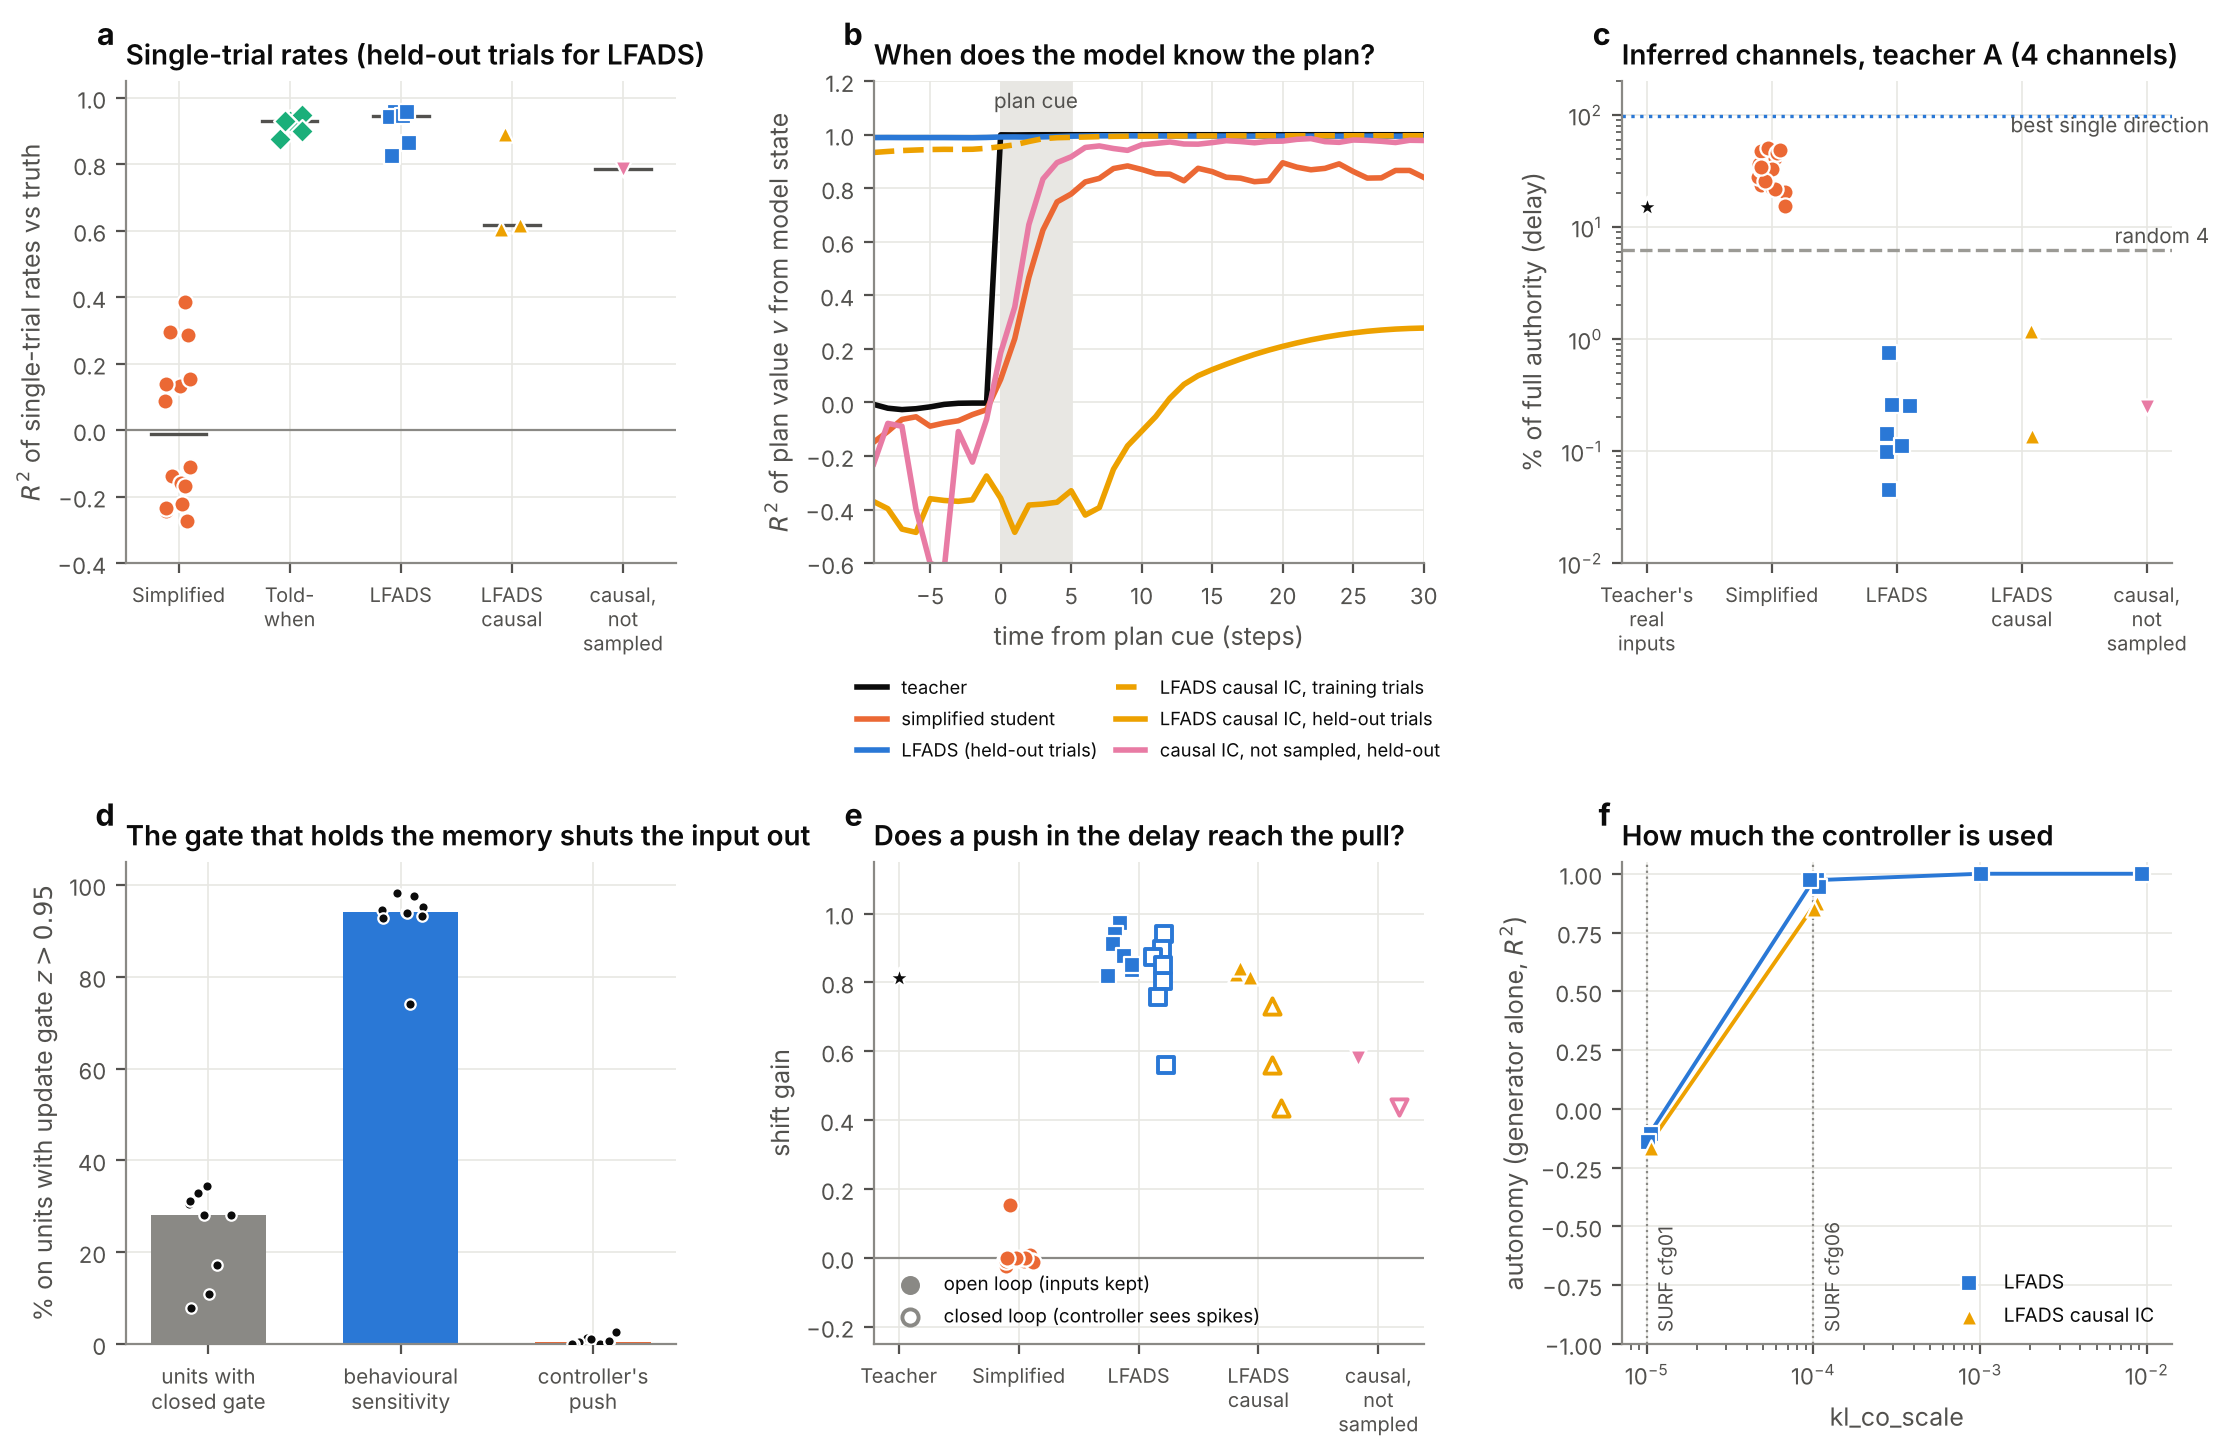
\includegraphics[width=\linewidth]{fig13_lfads.png}
  \caption{Full LFADS fitted to teacher A (held-out trials unless stated). (a) Accuracy of single-trial rates against the true rates. (b) When the model knows the plan: cross-validated $R^2$ of the plan value from the model state, aligned on the plan cue (grey). Standard LFADS knows it from the first step; the causal-IC model knows it on training trials only (dashed), by recognising them. (c) Delay-period authority of the four inferred channels, as a share of pushing on every unit (log scale). (d) In the delay, units with a closed update gate carry almost all the behavioural sensitivity but almost none of the controller's push. (e) Shift gain in open loop (filled) and closed loop (open symbols). (f) Autonomy against \kl{}.}
  \label{fig:lfads}
\end{figure}

\subsection{The inferred channels of full LFADS cannot reach its memory}\label{sec:res-lfads-auth}

In the delay, the four inferred channels of standard full LFADS have 0.04--0.8\% of full authority over the pull, against 6\% for four random directions and 92--98\% for the single best direction (\cref{fig:lfads}c). This is 8 to 150 times \emph{below} random, and 20 to 1000 times below the free students' 15--51\%. With the fair effort cost, an LQR controller acting through these channels removes 0.4--6\% of the error. This is the order of the 0.1\% found in SURF, and unlike with the free student (\cref{sec:res-goal}) it needs no special controller setting. The result holds for every variant (causal IC, not sampled; at most 1.2\%) and every \kl{} we tried (\cref{fig:lfads2}a), for teachers B and A2 and for a teacher with noise in its dynamics (\cref{fig:lfads2}b), and on MC\_Maze, where LFADS's inferred channels have 0.28--0.46\% of the authority over the reach, against 6\% for random and 100\% for the best four, so that LQR removes 2.5--4\% of the error (\cref{fig:lfads2}d; four fits).

The reason is the gated generator. A GRU unit keeps its value when its update gate $z$ is close to 1, and the same gate scales the effect of any input on that unit by roughly $(1-z)$ (\cref{app:faq}). A unit that holds the plan through the delay is therefore a unit the inputs cannot reach. In the delay only 8--34\% of the generator's units have $z>0.95$, but they carry 74--98\% of the behavioural sensitivity and receive only 0--3\% of the controller's push (\cref{fig:lfads}d; held-out trials, nine fits). The memory and the input channels sit in different units. The same holds for the MC\_Maze fits: in the last 300\,ms of the delay, the 33--36\% of units with closed gates carry 79--90\% of the sensitivity of the reach and receive 1.3--1.8\% of the push. The not-sampled control rules out a simpler explanation, that the generator learns to ignore its controller because during training the controller feeds it random samples: without sampling the authority is still 0.25--0.38\%.

This is a property of the model class, not of the circuit. The teacher is a plain $\tanh$ network, in which an input reaches every unit whatever the unit is holding, and its real inputs keep 15\% of full authority in the delay. The free student is the same kind of network, and its channels reach 15--51\%. The model used in SURF was a GRU, like the one here.


\begin{figure}[t]
  \centering
  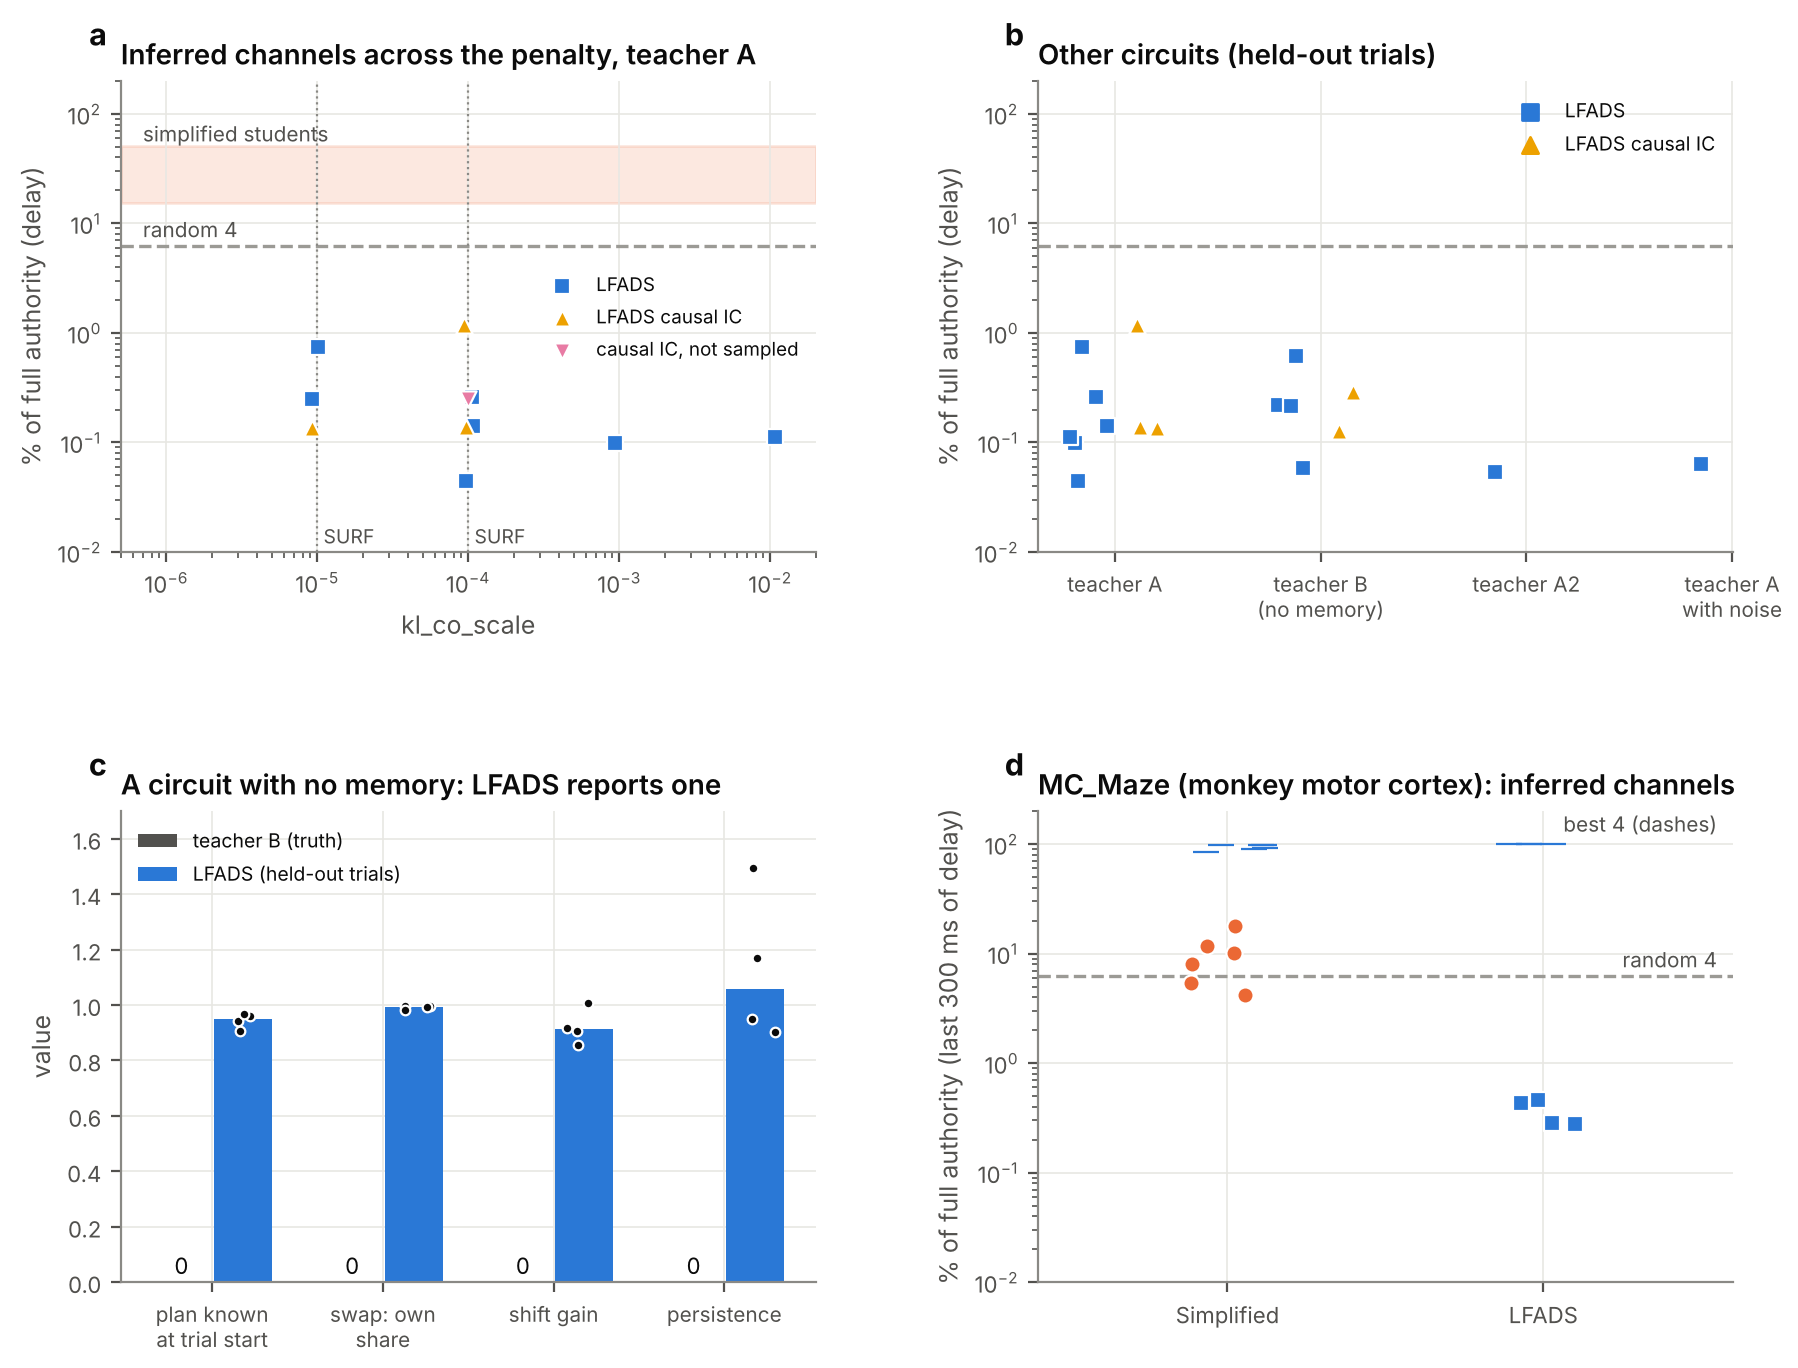
\includegraphics[width=0.92\linewidth]{fig14_lfads_robust.png}
  \caption{Robustness of the full-LFADS results. (a) Authority of the inferred channels against \kl{} (teacher A); orange band: free students. (b) Other teachers, including teacher A with noise in its dynamics. (c) Teacher B has no memory, but standard LFADS knows the plan from the first step and holds it like an attractor. (d) MC\_Maze: inferred channels of the free student and of full LFADS, with the best four (dashes) and random (dashed line).}
  \label{fig:lfads2}
\end{figure}

\subsection{Where full LFADS keeps the plan}\label{sec:res-lfads-plan}

Unlike the free student, full LFADS does hold the plan in its dynamics. On held-out trials a swap leaves the pull following the trial's own plan (open-loop own share 0.99--1.01, truth 1.00), a shift in the delay reaches the pull (gain 0.82--0.97, truth 0.81), and one direction persists over 20 steps (0.87--1.05, truth 0.99). Where fixed points were found (three of seven fits), the fixed-point analysis still reports 13--21 marginal directions out of 64, where the teacher has one.

But the model knows the plan too early (\cref{fig:lfads}b). The plan value can be read from the standard model's state at the first time step with $R^2=0.96$--0.99, before the plan cue has happened, on trials the model was never trained on. The teacher's $R^2$ there is 0. The initial-condition encoder reads the whole trial, including the plan cue and the pull, and writes the plan into the initial state, and the generator holds it from the start. The controller is not needed for the plan, which is why it can be switched off.

For teacher B, which has no memory, this produces a memory that is not there (\cref{fig:lfads2}c). In four fits (three seeds at $10^{-4}$, one at $10^{-5}$), standard LFADS again writes the plan into the initial state ($R^2=0.91$--0.97 at the first step) and holds it: own share 0.98--1.00, shift gain 0.85--1.01, persistence 0.90--1.49 (above 1, a slightly unstable direction), against 0.00 for all three in the teacher; the fit where fixed points were found has 18 marginal directions. Every test then reports an attractor holding the plan in a circuit that has none, and the three seeds agree with each other on it (generator states predict each other with $R^2=0.97$).

With the causal IC the plan cannot enter the initial state legitimately, and the result depends on the penalty. At $10^{-5}$ the controller delivers the plan at the cue and the generator holds it (held-out trials: plan not readable before the cue, $r=0.99$, open-loop own share 0.79). At $10^{-4}$ the model found a shortcut. On training trials the plan is readable from the first time step ($R^2=0.92$), although the encoder sees only the first 8 steps, which carry no information about the plan (the plan cannot be decoded from those spikes directly). The encoder learned to recognise each training trial from the noise in its first 160\,ms and to recall that trial's plan. On held-out trials this fails: the pull barely follows the plan ($r=0.26$) and the rates are poor ($R^2=0.61$). The same happened with a second seed (plan readable at the first step of training trials with $R^2=0.89$; on held-out trials $r=0.28$) and on teacher B. Training with the controller's mean instead of a sample removed the shortcut (\cref{fig:lfads}b, pink). An analysis of a fitted LFADS model should therefore be run on held-out trials.

Only one setting separated the two circuits: the causal IC at $10^{-5}$, tested on held-out trials. There the swap test gave an own share of 0.79 for teacher A and $-0.08$ for teacher B (truth 1.00 and 0.00), so the model of teacher B did take the plan from its controller through the delay. Even this model of teacher B had a persistent direction (0.96 after 20 steps) and responded to a shift (gain 0.60), where the teacher has neither, and on its training trials it again recalled the plan from the first step ($R^2=0.94$). In this setting the swap test was the only one of our tests that gave the right answer for both teachers.

\paragraph{Closed loop is not a simulator} When the controller stays in the loop, it keeps reading the real spikes and corrects the state toward them. Where the controller is used, a shift in the delay that persists in open loop is partly undone in closed loop (gain 0.56--0.76 against 0.84--0.97 for the standard model at $10^{-5}$, 0.56 against 0.84 with the causal IC; \cref{fig:lfads}e). In a closed-loop swap the controller writes the partner's plan into the state (own share 0.42--0.59 for the standard model, 0.19 with the causal IC). A fitted LFADS model with its controller running is a state estimator that follows the recordings, not a model of how the circuit would respond to stimulation; only the generator run in open loop can play that role.

\subsection{Does noise in the circuit help?}\label{sec:res-noise}

Off-attractor fluctuations could in principle tell a model how the circuit relaxes after a push \citep{galgali2023}. We generated recordings from teacher A with noise in its own dynamics (standard deviation 0.1 per step on every unit's input, which makes the trial-to-trial error of the pull about four times larger). This did not help. Full LFADS fitted to these recordings behaves as before (plan in the initial state, inferred channels 0.06\% of full authority), and the transfer of the model's best push to the teacher (\cref{sec:transfer}) stays at 5\% for LFADS and 0--7\% for two free students, against the 87\% ceiling. Across all full LFADS fits of teacher A the transfer reaches 1--14\%, so a much better fit does not by itself tell us where to push the circuit.

% ==================================================================== 5 DISCUSSION
\section{Discussion}\label{sec:discussion}

\Cref{tab:verdict} and \cref{fig:summary} summarise the evidence for each explanation of the 0.1\%.

\begin{table}[t]
  \centering
  \caption{Explanations for the 0.1\% and the evidence for each.}
  \label{tab:verdict}
  \small
  \begin{tabularx}{\linewidth}{@{}>{\raggedright\arraybackslash}p{3.6cm}>{\raggedright\arraybackslash}p{2.0cm}>{\raggedright\arraybackslash}X@{}}
    \toprule
    Explanation & Verdict & Main evidence \\
    \midrule
    Too few channels & Not\newline supported & One well aimed channel has 100\% of full authority on the teacher; the best four have 84--100\% on MC\_Maze; adding inferred channels does not close the gap. \\
    Inferred channels aimed arbitrarily & Supported & Simplified student: 15--51\% against 56--100\% for the best channels, threefold seed spread; on MC\_Maze 0.7--2.9 times random. \\
    Gated generator shuts its inputs out of its memory & Supported\newline (full LFADS) & Inferred channels 0.04--0.8\% of full authority, below random (6\%); LQR removes 0.4--6\% at a fair effort cost; 74--98\% of the sensitivity on closed-gate units, which get 0--3\% of the push; MC\_Maze 0.3--0.5\%. \\
    Model does not hold the plan as the circuit does & Supported & Simplified student: swap own share $-0.01$ to 0.06 (truth 1.00), shift gain 0.00 (truth 0.81). Full LFADS holds the plan, but writes it into the initial state before the cue, and does so for a circuit without memory. \\
    Circuit's own inputs miss the plan & Partly & Real inputs have 15\% of full authority in the hold, but still remove 57\% of the error. \\
    Goal was the whole state & Plausible & Whole-state goal scores real, random and best channels at 13--14\%; depends on the SURF target. \\
    Effort cost far too high & Possible & For the simplified student, 0.1\% needs $\rho$ 300--10\,000 times the fair value; full LFADS gets within a factor of 4--60 of 0.1\% without it. \\
    \bottomrule
  \end{tabularx}
\end{table}

\begin{figure}[t]
  \centering
  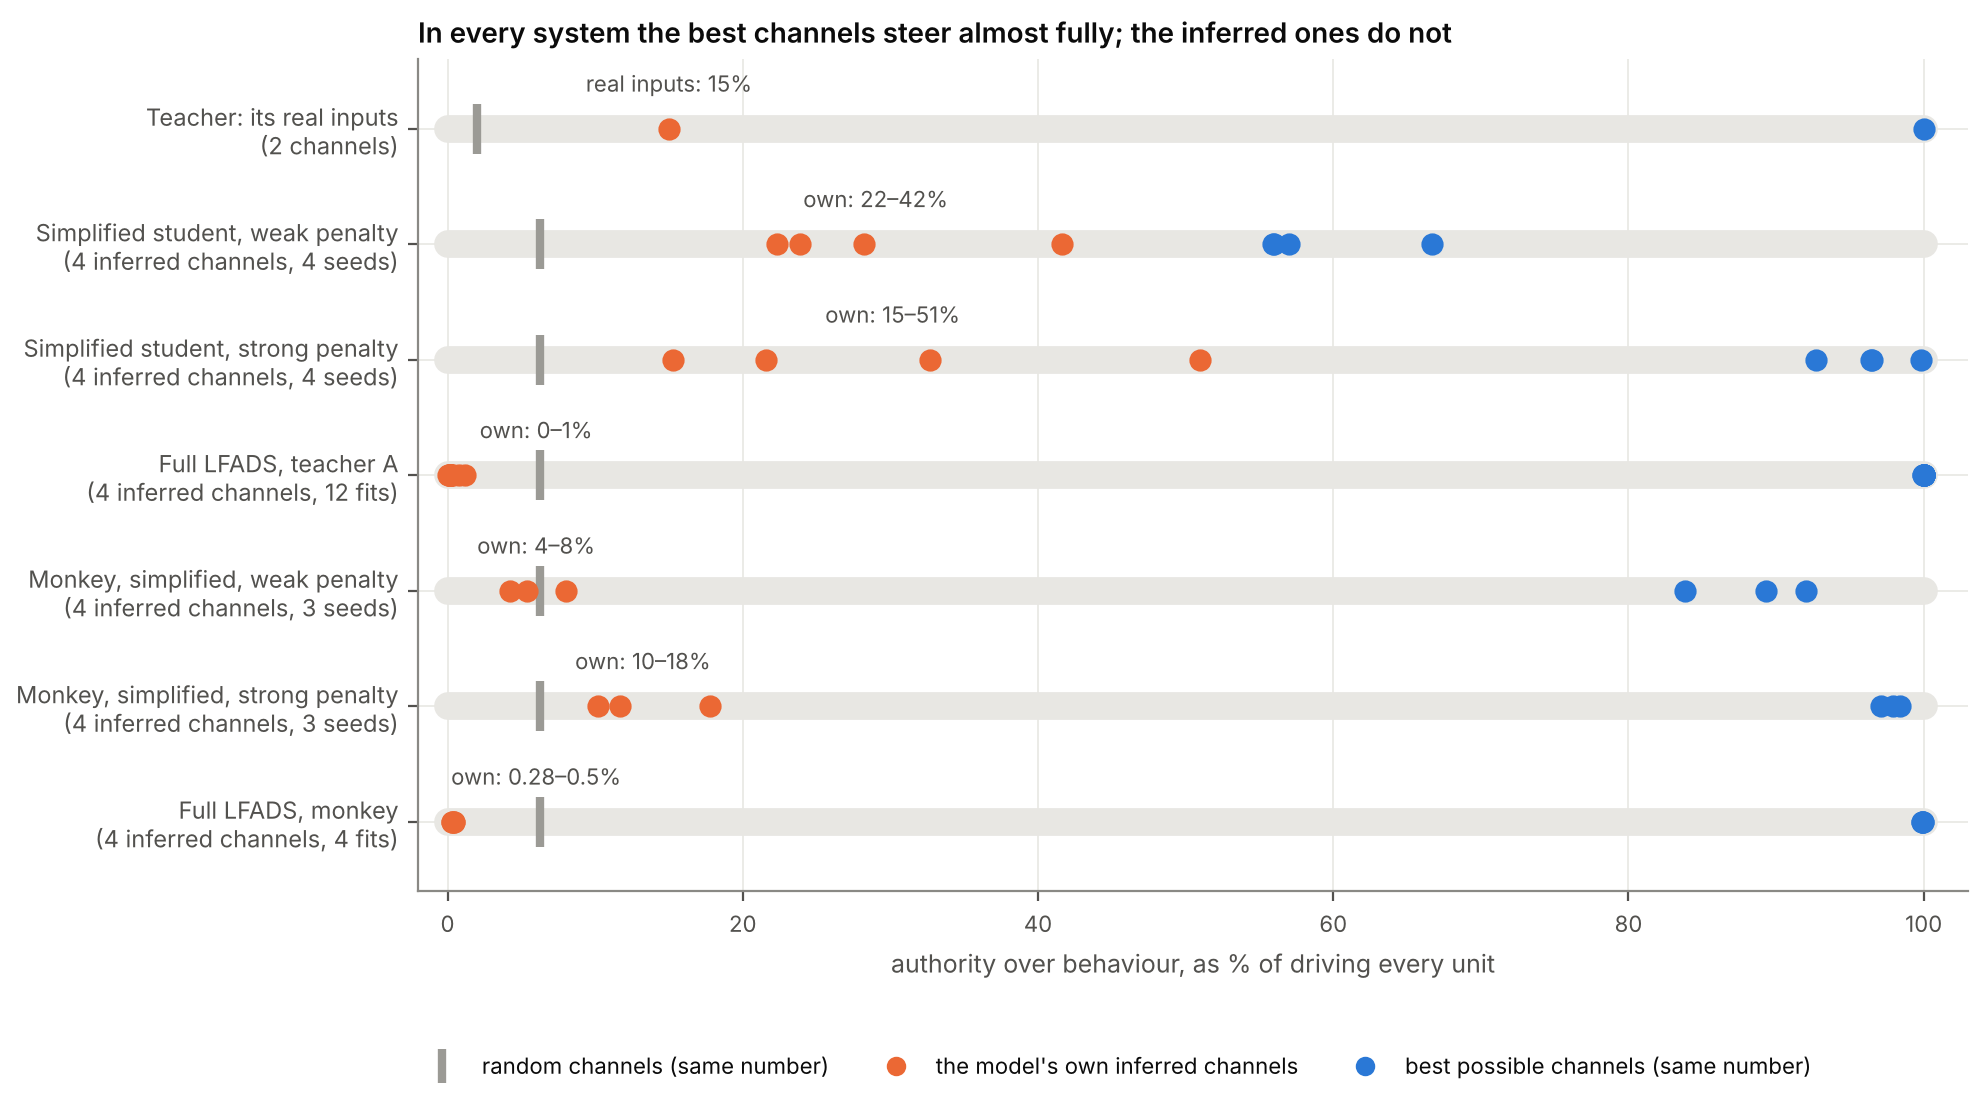
\includegraphics[width=0.8\linewidth]{fig11.png}
  \caption{The steering result in one picture. In every system the best channels of a given number (blue) have almost full authority over behaviour, while the inferred channels (orange; for the teacher, its real inputs) sit far below, and in the monkey model close to random (grey).}
  \label{fig:summary}
\end{figure}

\paragraph{What this means for the SURF result} Full LFADS at the SURF setting (\kl{} $=10^{-4}$) reproduces the SURF observations together: a nearly autonomous generator (94--97\%, against 97\% and 87\% in SURF), many marginal directions where fixed points could be found, and inferred channels through which an LQR controller with a fair effort cost removes 0.4--2.3\% of the error, against 0.1\% in SURF. Unlike with the simplified student, no unusual controller setting has to be assumed. The cause is a property of the model and not of the cortex: a gated generator holds its memory in units its inputs cannot reach, so steering through the controller's channels is close to impossible by construction. In addition, the SURF model's initial-condition encoder read each whole trial, so its state probably carried trial-specific information from the first time step. The 0.1\% therefore says little about how controllable M1 is. Two checks on the SURF model would settle this in minutes, without new recordings: compare the authority of its inferred channels with random channels of the same number (\cref{fig:lfads}c), and decode the trial's behaviour from the model state before the cue (\cref{fig:lfads}b). The marginal count of 33/128 is the kind of count fitted generators produce with one slow direction or none (\cref{sec:res-marginal,sec:res-lfads-plan}), so it does not by itself establish an attractor in M1, nor exclude one. The behavioural-axis value of 0.352 is also what a perfectly steerable line attractor gives (\cref{sec:res-axis}).

\paragraph{Internal memory or outside input} How much activity a model attributes to its dynamics and how much to inputs is set by its assumptions, here the controller's freedom. This ambiguity is known \citep{sussillo2016,malonis2026,versteeg2025}; our contribution is to show its consequences with the truth known. A free student turns an attractor into controller input, a told-when student turns a sustained input into an attractor, both fit the spikes, and the one with the wrong mechanism can predict held-out neurons better (\cref{fig:grid}). On MC\_Maze the same model family places the reach in the initial state or in the controller depending on the number of channels. Full LFADS gives a third answer: the plan is written into the initial state by an encoder that has read the whole trial, and then held by the generator, so it reports an attractor for teacher B, which has none. A claim such as ``push along this direction and the plan will move and stay moved'' concerns the circuit's own dynamics, and a model fitted to recordings alone supports it only if its split is right. The split must be checked with a perturbation.

\paragraph{Relation to ensemble diagnostics} \citet{malonis2026} found that sustained inputs never reached ensemble agreement in their simulations, and proposed agreement across an ensemble of fits as a diagnostic. Our results show that agreement and correctness can come apart. Three full LFADS fits of teacher A with different seeds agree almost perfectly on their generator states (cross-validated $R^2=0.97$ between fits), although all three load the plan at the wrong time, and three fits of teacher B agree just as well ($R^2=0.97$) on a memory that teacher B does not have. Of the six told-when fits of teacher B, the two that carried the plan both did it with an invented memory. The free students, in contrast, agree poorly with each other (states 0.15--0.35, inferred inputs 0.15--0.21) although each one's state contains the teacher's state ($R^2$ 0.78--0.89 from fit to teacher). Agreement measures how strongly the data and the assumptions together fix the answer, not whether the assumptions are right.

\paragraph{Practical message} For stimulation experiments, the results suggest not pushing along inferred channels and not simply adding channels. The direction that matters is the one behaviour is most sensitive to, which on the teacher is the left eigenvector of the slow mode, $24^\circ$ off the attractor. No fitted model recovered that direction for the true circuit (\cref{sec:res-transfer,sec:res-noise}), not even full LFADS with an excellent fit, so a small number of calibration perturbations is probably worth more than a better fit to recordings. If a fitted LFADS model is used to plan stimulation, its generator state should be pushed directly, or a generator without gates should be used, rather than its controller channels; and it should be analysed on held-out trials and in open loop.

\subsection{Limitations}\label{sec:limitations}

The teachers are small networks on an idealised task; the SURF mouse task has no plan cue and a roughly fixed pull (\cref{app:faq}). Most analyses use a simplified LFADS that fits each trial's initial state and inputs directly with an $L_2$ penalty. Its single-trial rates are far from the truth ($R^2$ below 0.4), because its free inputs also fit spike noise, so its fitted generator is a poor copy of the teacher's dynamics. We therefore repeated the central tests with full LFADS (\cref{sec:res-lfads-fit,sec:res-lfads-auth,sec:res-lfads-plan}), which fits well. Our LFADS is smaller than SURF's (64 against 128 generator units), it was trained for a fixed number of steps without a hyperparameter search, and we ran one to three seeds per setting. The gate explanation should apply to any gated generator, but we did not test other architectures. The told-when student is given that nothing else arrives, which is the point in question; we use it to show the effect of the opposite assumption, not as a better model. On MC\_Maze our held-out scores (0.13--0.145 bits per spike for the simplified student, 0.22 for full LFADS) are below published LFADS results, which use different bins, windows and test sets, and MC\_Maze is one session from one monkey. The steering analysis assumes small pushes (valid to about 0.1 change in pull). The penalty sweep in \cref{fig:aim}a is one seed per setting. Four simplified fits failed numerically and were refit or excluded, as stated in each case. We did not reproduce the SURF controller, whose target, effort cost and horizon are unknown, and we did not run the new tests on the SURF model, since it was fitted to laboratory data.

% ==================================================================== 6 CONCLUSION
\section{Conclusions and future work}\label{sec:conclusion}

\begin{enumerate}
  \item The SURF 0.1\% was not caused by having too few channels: one well aimed channel suffices on the teacher, and four suffice in models of monkey motor cortex.
  \item Inferred channels are poorly aimed for steering. In the simplified student they reach 15--51\% of the available authority. In full LFADS they reach 0.04--0.8\%, below random, on every teacher and on MC\_Maze, because the update gate that holds the generator's memory also shuts its input out. An LQR controller acting through them removes 0.4--6\% of the error at a fair effort cost, the order of the SURF 0.1\%.
  \item The best push is the left eigenvector of the slow mode, $24^\circ$ off the line of states. Mean-difference axes and ridge decoders cannot find it, and no fitted model recovered it for the true circuit, even with noise in the circuit's dynamics.
  \item Fitted models do not keep the plan as the circuit does. The simplified student is handed the plan by its controller at the go cue; full LFADS writes it into its initial state before the plan cue, and so reports an attractor even for a circuit that has none. Fixed-point analysis finds many marginal directions in all of them.
  \item The mechanism a model reports follows its assumptions. Held-out prediction and agreement across seeds do not choose between them; a perturbation does.
  \item Fitted LFADS models should be analysed on held-out trials and in open loop: on training trials a causal LFADS recalled each trial's plan from noise, and with its controller running LFADS undoes perturbations.
  \item The 0.1\% most likely came from the fitted model rather than the cortex. Comparing the SURF model's inferred channels with random ones and decoding behaviour from its state before the cue would confirm this.
\end{enumerate}

\paragraph{Future work}
(1) Repeat the full-LFADS tests at the SURF size (128 generator units), with a hyperparameter search and five or more seeds per setting, and with a generator without gates, to check that the channels then regain authority. (2) Run the two checks above on the SURF model. (3) Work out the linear theory of which models are equivalent given the recordings, and which assumptions (known input timescale, sparse inputs, a causal encoder) select one. (4) Find the cheapest perturbation that separates internal memory from external input, and test whether a few perturbation trials added to training fix the model's mechanism. (5) Build a teacher closer to the mouse task and extend the public-data test to more sessions, benchmark tasks with known inputs \citep{versteeg2025} and a mouse dataset with cued forelimb movements.

\section*{Acknowledgements}
I thank Prof.\ Amitabha Nandi for supervising this project. The question grew out of a summer internship in Prof.\ Krishna Jayant's Nano Neurotechnology Lab at Purdue University, mentored by Om Kolhe. No data from that laboratory is used here; all results use simulated networks and the public MC\_Maze dataset of the Neural Latents Benchmark.

\bibliographystyle{plainnat}
\bibliography{refs}

% ==================================================================== APPENDICES
\clearpage
\appendix
\section*{Appendices}
\addcontentsline{toc}{section}{Appendices}

\section{Derivation of the authority--LQR identity}\label{app:derivation}

\paragraph{Linearity} For small pushes, $\Delta\pull = \sum_t \vect s_t^\top \vect x_t$ (a first-order Taylor expansion); \cref{fig:teacher-steer}c shows this holds to within 10\% for changes up to about 0.1.

\paragraph{Restriction to channels} With channels $B$ the push is $\vect x_t = B\vect u_t$, so $\Delta\pull = \sum_t (B^\top \vect s_t)^\top \vect u_t$. Only the part of the sensitivity the channels see, $B^\top\vect s_t$, matters.

\paragraph{The cheapest push} For a given $\Delta\pull$, the effort $\sum_t\lVert\vect u_t\rVert^2$ is minimised by $\vect u_t = c\,B^\top\vect s_t$ (Cauchy--Schwarz). Then $\Delta\pull = cG$ and the effort is $c^2G$, with
\begin{equation}
  G = \sum_t \lVert B^\top\vect s_t\rVert^2 = \tr(B^\top Q B).
\end{equation}

\paragraph{The optimal strength} LQR minimises $J(c) = (T - cG)^2 + \rho\,c^2G$ for a target change $T$. Setting $dJ/dc = -2G(T-cG) + 2\rho cG = 0$ gives
\begin{equation}
  c^* = \frac{T}{G+\rho}, \qquad \frac{c^*G}{T} = \frac{G}{G+\rho},
\end{equation}
which is \cref{eq:lqr}. For a single unit-norm channel $\vect b$ at angle $\theta$ to the top eigenvector of a rank-one $Q$, $G = \cos^2\theta\,\tr Q$, which is why authority behaves as $\cos^2\theta$ (\cref{fig:a-authority}).

\paragraph{Random baseline} For $k$ random orthonormal directions in $\mathbb R^N$, $\mathbb E[BB^\top] = (k/N)I$, so $\mathbb E[G] = (k/N)\tr Q$. For $N=100$ and $k=1$ the fraction has mean 1\% and standard deviation about 1.4\%; only 2.5\% of random directions exceed 5\%.

\section{A two-unit example of non-normal steering}\label{app:nonnormal}

Take $a_{t+1} = a_t + b_t$, $b_{t+1} = 0$. The resting states are $(a,0)$, so the line of states (right slow eigenvector) is $(1,0)$. A unit push along the line leaves $a=1$. A push of the same size along $(1,1)/\sqrt2$ leaves $a = 2/\sqrt2 \approx 1.41$ after one step, because $b$ feeds into $a$ before it decays. The best direction is the left eigenvector $(1,1)/\sqrt2$, $45^\circ$ from the line. If $b$ did not feed into $a$, the system would be normal and the best push would lie along the line. In the teacher the corresponding angle is $24^\circ$.

\section{Model and analysis details}\label{app:details}

\begin{table}[h]
  \centering
  \caption{Parameters.}
  \label{tab:params}
  \small
  \begin{tabularx}{\linewidth}{@{}p{3.8cm}X@{}}
    \toprule
    Teachers & 100 tanh units; inputs: plan, go; outputs: lever and a training-only plan report; gain 0.9; activity noise 0.05 in training; 150-step trials; $v\sim\mathcal U(0.2,1)$; delay 35--85 steps; 6000 Adam steps. Teacher A and A2: 5-step plan pulse; teacher B: plan on until go. Final lever MSE (A) $5.7\times10^{-5}$. \\
    Synthetic data & 256 trials; 60 Poisson neurons (50 fit, 10 held out); log-rate gain $\sigma=0.7$; baselines 0.08--0.45 spikes/step; no dynamics noise. \\
    Free student & 64 tanh units, 12 factors, $k$ unit-norm channels; per-trial $\vect g_0$ and $\vect u_t$; Poisson likelihood; penalty $\lambda\,\overline{u^2}$; $10^{-5}\lVert W\rVert^2$; Adam, learning rate $10^{-2}$, cosine schedule, 2500 steps. \\
    Full LFADS & lfads-torch modules; generator GRU 64, controller GRU 32, 4 controller outputs, 12 factors, IC 32, IC and CI encoders 32 per direction, CI lag 1; IC prior Gaussian (variance 0.1), CO prior AR(1) ($\tau=10$, variance 0.1, learned); recon loss scale $10^4$; KL and $L_2$ ($10^{-4}$, generator and controller) ramped over the first 600 steps; dropout 0.1, coordinated dropout 0.3, cell clip 5; Adam $4\times10^{-3}$, batch 64, 3000 steps, decay after step 1800; 192 training and 64 held-out trials (fixed split); causal IC: IC encoder on the first 8 steps. MC\_Maze: all 366 trials, same settings. \\
    Told-when student & Same generator and readout; shared $\vect g_0$; go waveform lags $-3$ to $+11$; two load waveforms lags $-1$ to $+6$ with two amplitudes per trial; 7000 steps. \\
    Pull and decoder & Pull: mean lever over steps $t_{\mathrm{go}}+8$ to $t_{\mathrm{go}}+27$. Students: ridge decoder from generator state to the teacher's lever (ridge $10^{-2}$; $R^2$ 0.52--0.88); aim changes by less than 0.06 for ridge $10^{-4}$ to 1. \\
    Steering & Sensitivities by back-propagation; load window: 5 pulse steps; delay window: 30 to 5 steps before go; 200 random channel sets; $\rho$ set so full actuation removes 90\%; medians over trials. \\
    Whole-state goal & State 5 steps before go; exact Jacobian to delay pushes; random targets; 64 trials. \\
    Plan tests & Swap from 8 steps after the plan pulse, random partners aligned on go; shift 25 steps before go by $0.1\,\vect m$; persistence over steps $t_{\mathrm{go}}-30$ to $t_{\mathrm{go}}-10$, median over 32 trials; fixed points from 32 delay states, residual $<10^{-5}$, marginal $0.95<|\lambda|<1.05$. \\
    Transfer & 64 trials, delay window, immediate-effect matching on the 50 fitted neurons, pseudo-inverse cutoff $10^{-2}$. \\
    MC\_Maze & 20\,ms bins, $-300$ to $+800$\,ms around go, 366 trials, 137 neurons (103/34); log-rate cap, halved learning rate; reach end point over 400\,ms after movement onset. \\
    \bottomrule
  \end{tabularx}
\end{table}

\paragraph{Code} Everything runs on a CPU; a free-student fit takes 2--7 minutes, a told-when fit about 8 and a full LFADS fit 20--40, and about 150 fits were run in total.
\begin{itemize}[leftmargin=1.2em]
  \item \texttt{teacher.py}, \texttt{split\_study.py}: teachers A, A2 and B, and synthetic data.
  \item \texttt{lfads\_lite.py}: free student. \texttt{event\_student.py}: told-when student.
  \item \texttt{control.py}: Gramian and LQR identity. \texttt{steer.py}, \texttt{student\_steer.py}: steering analysis.
  \item \texttt{state\_target.py}: whole-state goal. \texttt{rho\_sweep.py}: effort-cost sweep.
  \item \texttt{plan\_tests.py}, \texttt{mc\_plan\_tests.py}: swap, shift and persistence. \texttt{fp\_count.py}: fixed points.
  \item \texttt{event\_tests.py}: told-when students and transfer. \texttt{mc\_maze.py}: public data.
  \item \texttt{lfads\_full.py}: full LFADS from the lfads-torch modules.
  \item \texttt{lfads\_tests.py} and \texttt{lfads\_mc\_tests.py}: all tests on full LFADS.
  \item \texttt{gate\_check.py}: update gates. \texttt{v\_timecourse.py}: when the plan is known.
  \item \texttt{ensemble.py}: agreement between fits. \texttt{make\_noisy.py}: teacher with dynamics noise.
\end{itemize}

\section{Supplementary schematics}\label{app:schematics}

\begin{figure}[h]
  \centering
  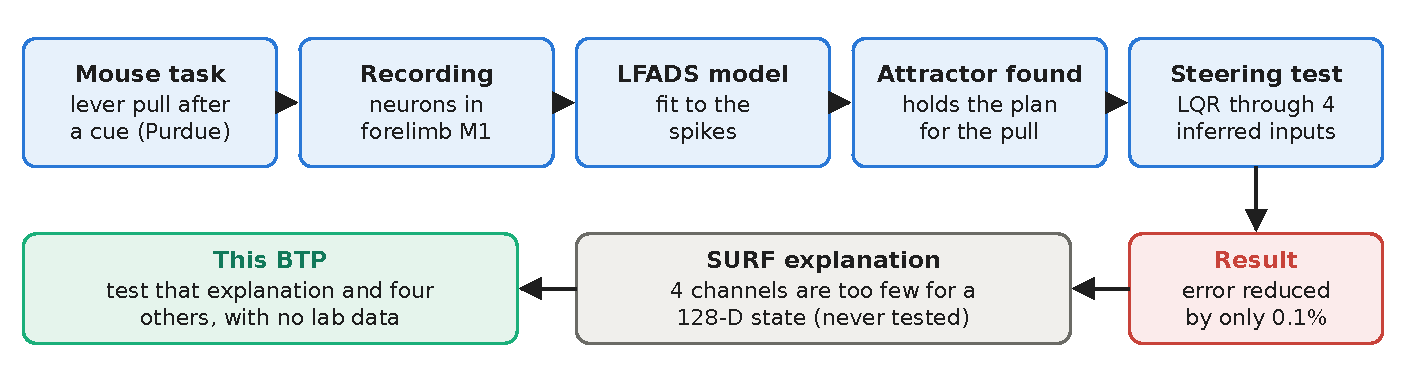
\includegraphics[width=0.9\linewidth]{d1_story.pdf}
  \caption{The SURF result and where this project starts.}
  \label{fig:a-story}
\end{figure}

\begin{figure}[h]
  \centering
  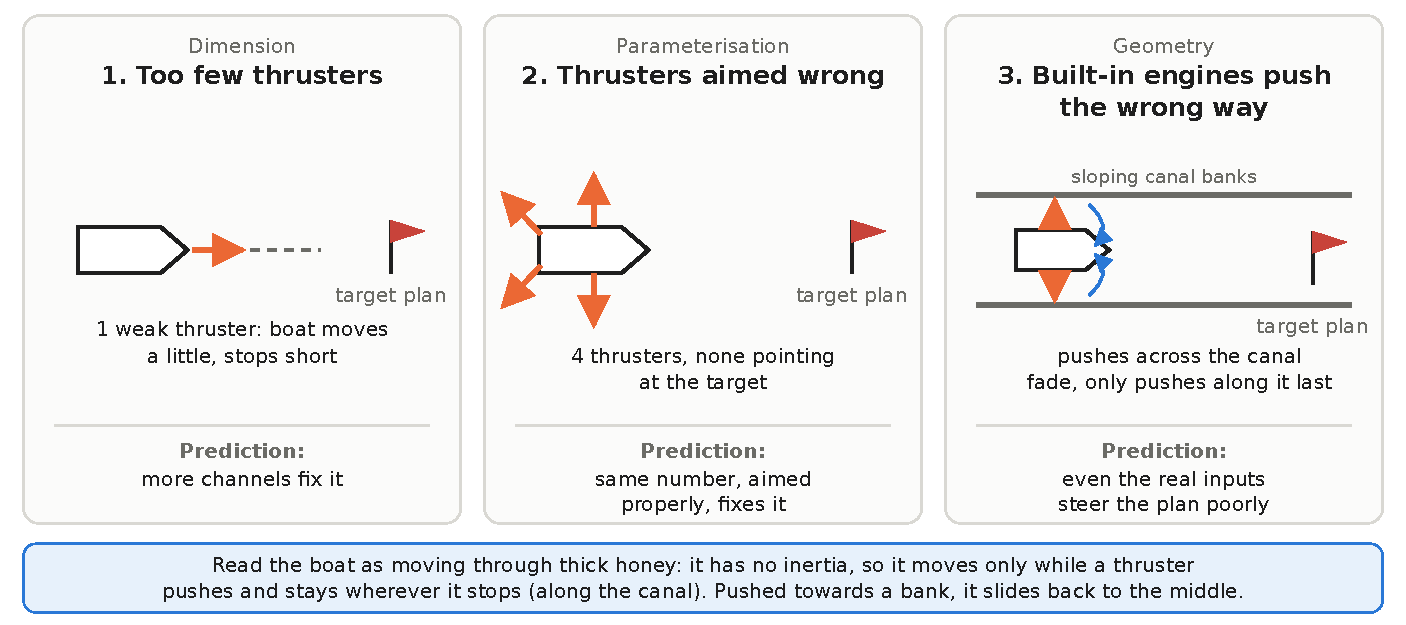
\includegraphics[width=0.95\linewidth]{d2_boats.pdf}
  \caption{The three explanations, with the plan as a boat in thick honey (it moves only while pushed and stays where it stops) and the channels as thrusters. Each predicts something different.}
  \label{fig:boats}
\end{figure}

\begin{figure}[h]
  \centering
  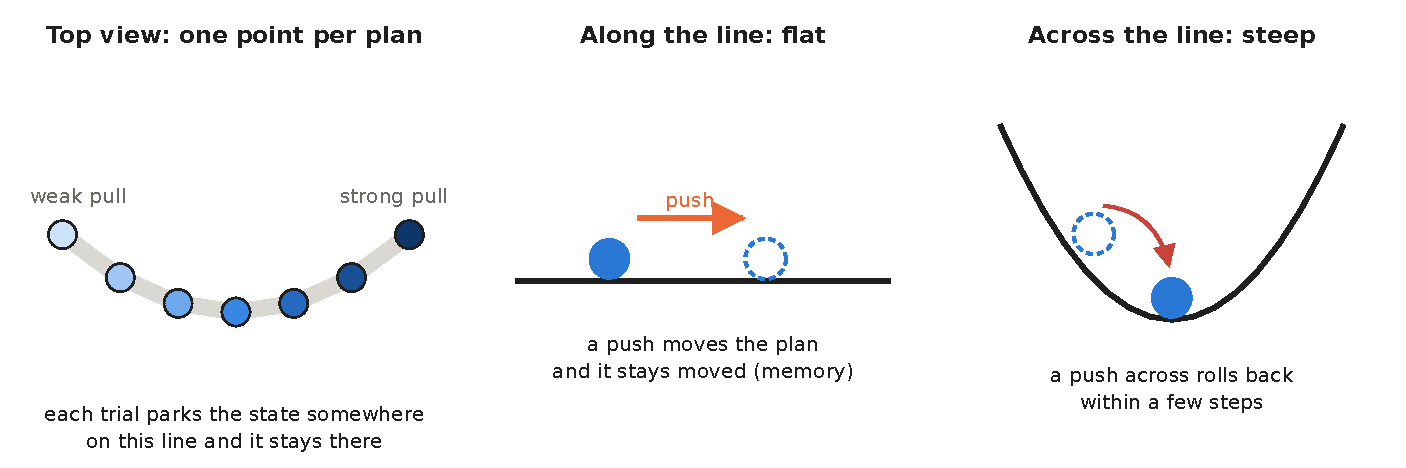
\includegraphics[width=0.85\linewidth]{d3_attractor.pdf}
  \caption{A line attractor: a push along the valley stays, a push across it rolls back.}
  \label{fig:a-attractor}
\end{figure}

\begin{figure}[h]
  \centering
  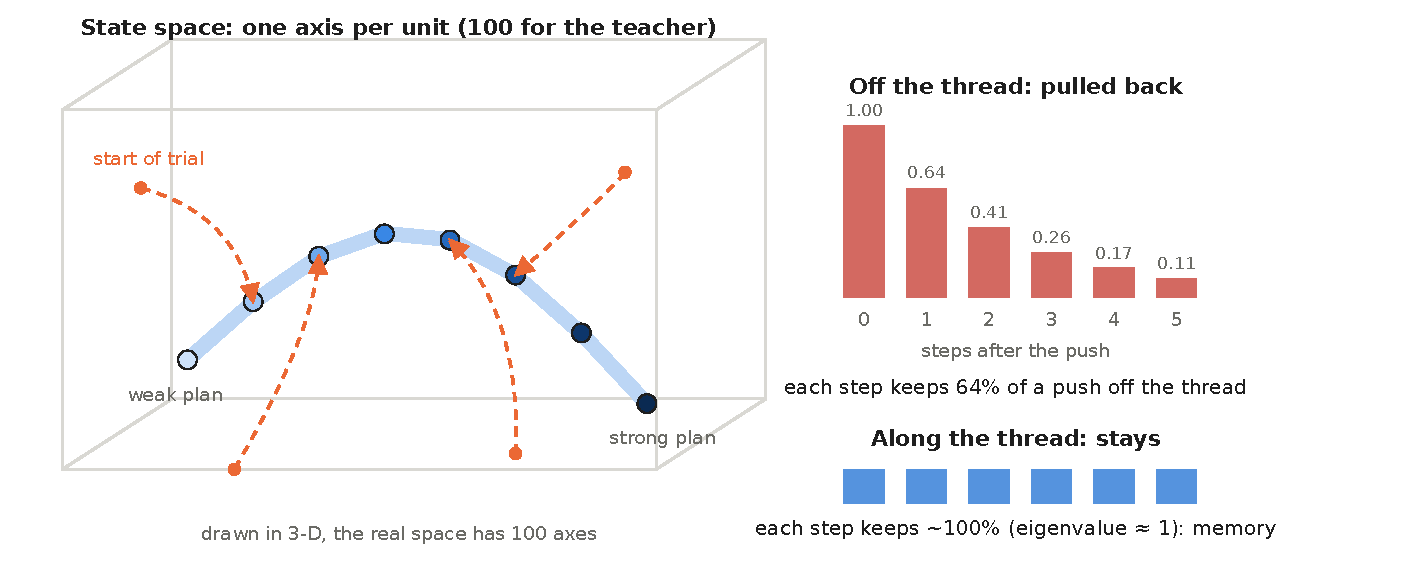
\includegraphics[width=0.85\linewidth]{d12_thread.pdf}
  \caption{A line attractor in a high-dimensional space: each trial rests on a thin curved thread at a position set by its plan.}
  \label{fig:a-thread}
\end{figure}

\begin{figure}[h]
  \centering
  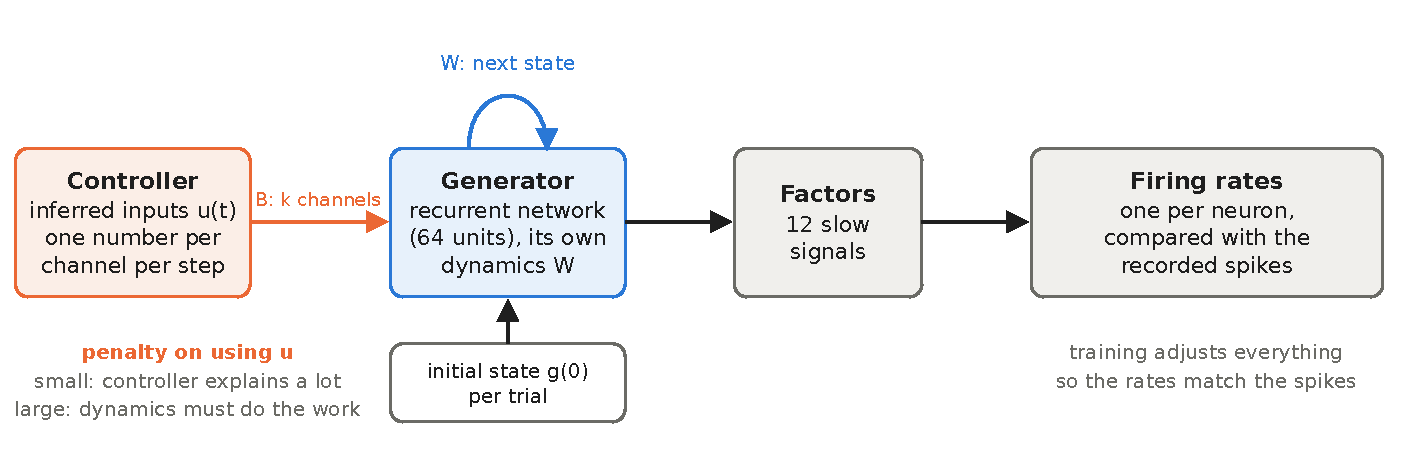
\includegraphics[width=0.9\linewidth]{d6_student.pdf}
  \caption{Inside the free student. The controller's inputs enter the generator through $k$ channels (the columns of $B$); the penalty decides how much the controller may explain.}
  \label{fig:a-student}
\end{figure}

\begin{figure}[h]
  \centering
  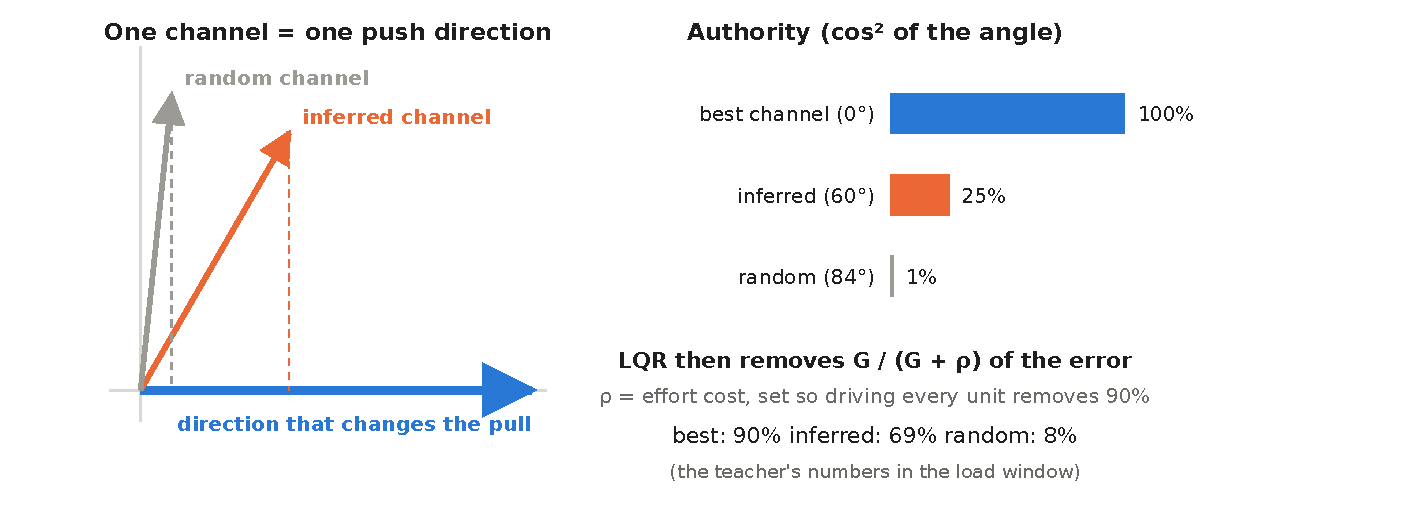
\includegraphics[width=0.9\linewidth]{d7_authority.pdf}
  \caption{Authority for one channel: only the part of a push along the sensitive direction counts, so a channel at $60^\circ$ has 25\% authority and a random channel almost none.}
  \label{fig:a-authority}
\end{figure}

\begin{figure}[h]
  \centering
  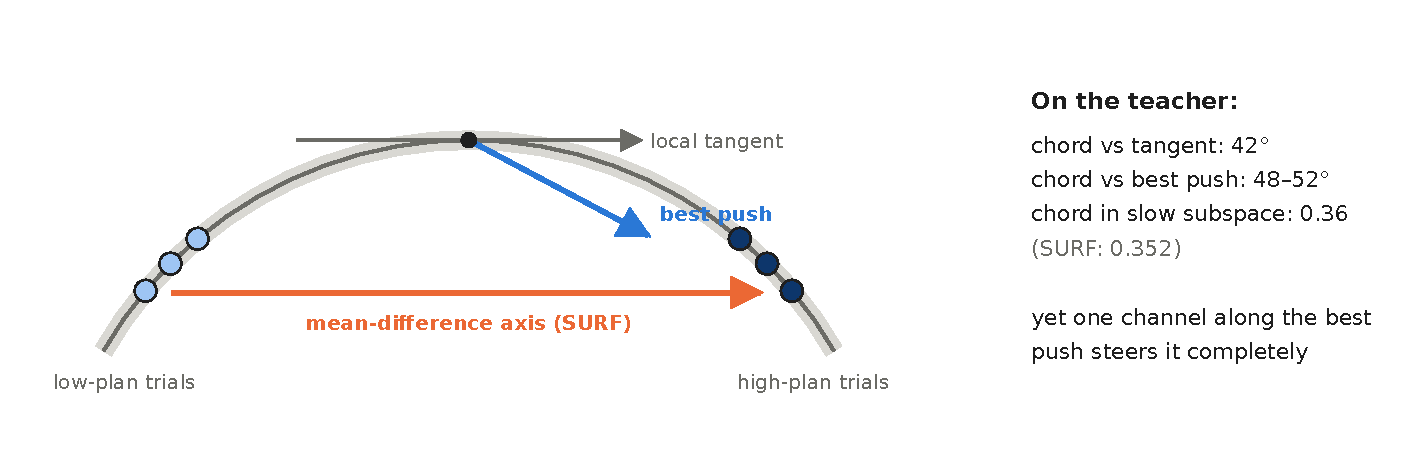
\includegraphics[width=0.85\linewidth]{d8_meandiff.pdf}
  \caption{On a curved line of states, the difference between two group means is a chord that points away from both the local tangent and the best push.}
  \label{fig:a-meandiff}
\end{figure}

\begin{figure}[h]
  \centering
  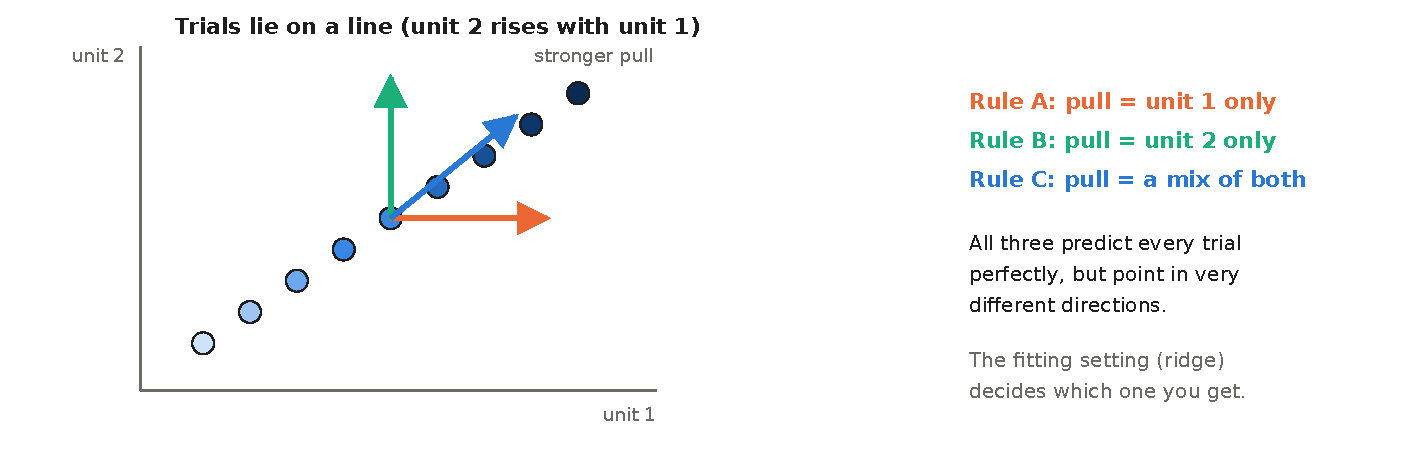
\includegraphics[width=0.85\linewidth]{d13_decoders.pdf}
  \caption{When trials lie on a line, several decoders predict them all perfectly, and the fitting setting picks one.}
  \label{fig:a-decoders}
\end{figure}

\begin{figure}[h]
  \centering
  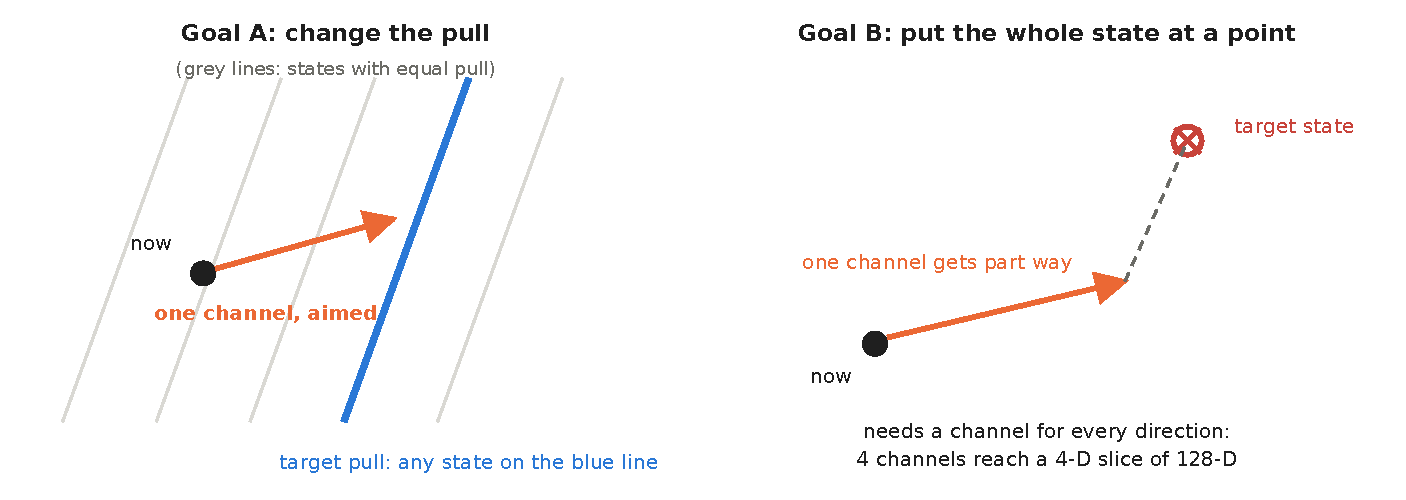
\includegraphics[width=0.85\linewidth]{d10_goals.pdf}
  \caption{Two goals for the controller: changing the pull needs the state to reach a line of equal pull, which one aimed channel can do; placing the whole state at a point needs a channel for every direction.}
  \label{fig:a-goals}
\end{figure}

\begin{figure}[h]
  \centering
  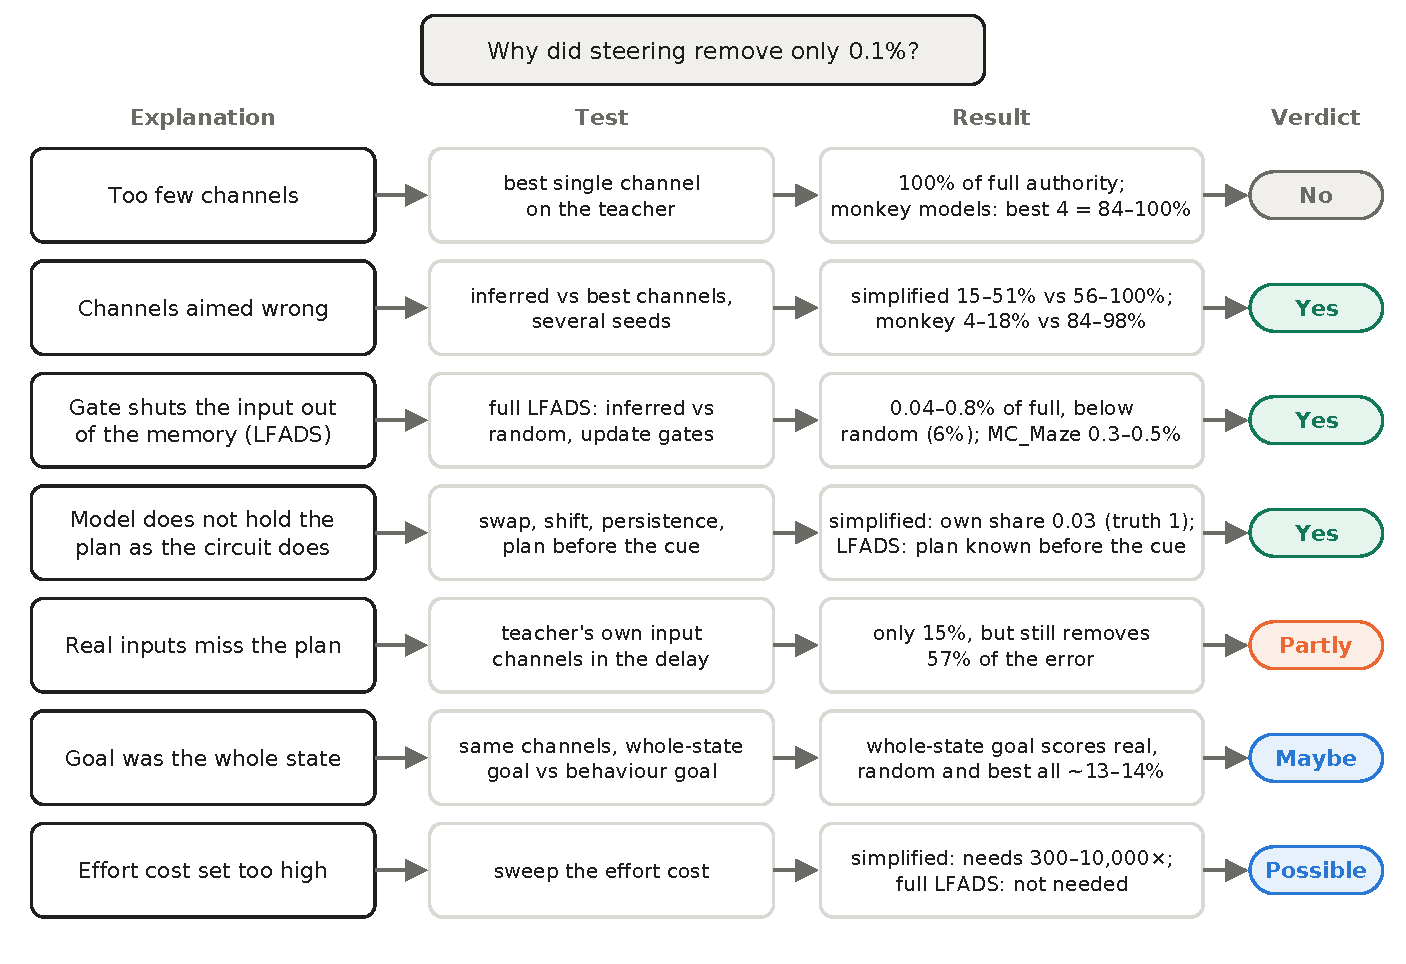
\includegraphics[width=0.9\linewidth]{d11_verdict.pdf}
  \caption{Each explanation, the test used, the result and the verdict.}
  \label{fig:a-verdict}
\end{figure}

\FloatBarrier
\section{Questions a reader might ask}\label{app:faq}

\paragraph{If inferred inputs are whatever the state cannot explain, how can they be bad at steering?} Explaining and steering are different jobs. Inferred inputs point wherever the generator's own dynamics fail to match the spikes, mostly at the go cue and in trial-to-trial noise. Steering asks in which direction a push now changes behaviour later, and nothing in the fit rewards that. In addition, the free student does not hold the plan during the delay (\cref{sec:res-plan}), so there is no held plan for its channels to be aimed at, and many channel directions explain the spikes equally well \citep{malonis2026}.

\paragraph{How can a circuit's own inputs miss its plan?} A memory is useful only if ordinary inputs do not disturb it. The teacher's inputs load the plan (25\% of full authority, 24 times random) and trigger the movement; during the hold, an input that moved the plan would corrupt the memory, so a trained network keeps its inputs mostly off the plan direction (15\%). Real circuits appear to do the same \citep{finkelstein2021,oshea2022}.

\paragraph{Why use a teacher and a student rather than only real data?} With real data the answer can never be checked. The teacher is like a phantom used to test a scanner: its insides are known, and the student plays the role LFADS played in SURF. The teacher is trained rather than hand-built because a trained network is imperfect in the ways that matter here: its line is curved, it leaks, and it is non-normal.

\paragraph{Why Poisson spikes?} Spike counts vary across repeats with variance roughly equal to the mean over short bins, which is the Poisson property, and LFADS assumes it. A Poisson count with mean 3 has a typical spread of $\sqrt3\approx1.7$, one with mean 10 a spread of about 3.2.

\paragraph{What does a score in bits per spike mean?} It is the log-likelihood gain over a constant-rate model, in bits, divided by the number of spikes. A score of 0.3 means each spike was on average $2^{0.3}\approx1.23$ times more probable under the model.

\paragraph{Why does a held value need a line attractor?} With no input during the delay, each plan needs its own resting state, and a continuum of plans needs a continuum of resting states. Alternatives are discrete attractors for a few plans \citep{inagaki2019}, a moving code read out by a matched decoder, or synaptic storage, which the teacher cannot use.

\paragraph{Is the mouse task comparable to the monkey task?} Not as a behaviour. The SURF task has no plan cue; the tone is the go signal and the pull is similar each time, so the waiting-period state more likely holds readiness and timing than a planned value. The comparison here is of the analysis pipeline: whether inferred channels are aimed in the direction that changes behaviour, a question that applies wherever pre-movement activity predicts the movement. A teacher closer to the mouse task is future work.

\paragraph{Why a simplified LFADS?} The quantity studied is the fitted generator and its channels, and about 100 fits were needed on a CPU; the simplified student made that possible. Full LFADS takes 20 to 40 minutes per fit at our sizes, so it was used for the central tests (\cref{sec:res-lfads-fit,sec:res-lfads-auth,sec:res-lfads-plan}). It changes one conclusion and strengthens another: full LFADS does hold the plan in its dynamics, but loads it too early, and its inferred channels are far worse aimed than the simplified student's.

\paragraph{Does this mean LFADS is wrong?} No. LFADS is built to denoise spikes and describe population activity, and it does that well here (single-trial rate $R^2$ about 0.95). The problems start when its parts are read as the circuit's parts: the controller as the circuit's input, the generator's slow directions as the circuit's attractor, and the controller's channels as the places to stimulate. Nothing in its training asks it to get these right.

\paragraph{Why does a GRU shut its input out of its memory?} A GRU unit updates as $g\leftarrow z\,g + (1-z)\,n$, where $n$ is the new candidate value, which depends on the input, and $z$ is the update gate. With $z$ near 1 the unit keeps its value, which is how a GRU remembers; but then the input, which acts only through $n$ and $z$, changes the unit by a factor $(1-z)$, close to zero. A plain $\tanh$ unit has no such gate: it forgets unless the recurrent weights hold the value, and an input always reaches it.

\section{Changes from the progress report}\label{app:changes}

\paragraph{Changes in the final version} The central tests were repeated with full LFADS (\cref{sec:lfads}), which changes two statements of the earlier draft. First, ``free LFADS-style models supply the plan through their controller'' holds for the simplified student only; full LFADS holds the plan in its generator but loads it into the initial state before the cue. Second, the earlier view that the 0.1\% needed an extreme effort cost or an unusual goal is no longer needed: full LFADS's channels give a number of that order with a fair effort cost. The told-when experiment now has five seeds on teacher A and six on teacher B (previously three each); on teacher B only two of six carried the plan, both with an invented memory. We also report that the simplified student's single-trial rates are far from the truth.


In the progress report, whether a student holds the plan was tested by switching its controller off during the delay only. The controller at and after the go cue stayed on, which is where the students place the plan, so the test passed for reasons unrelated to memory. The swap test replaces all inputs after the plan is loaded and does not have this gap. The following conclusions were therefore withdrawn: that low-penalty students hold the plan internally; that the students of teacher A recover the correct mechanism; and that the students of teacher B ``invent an attractor and wrongly predict that the plan survives''. Single-step eigenvalue magnitudes reported as slow were mostly rotating or sign-flipping directions. Measurements on the teachers, the authority comparisons and their seed dependence are unaffected.

\end{document}
